\documentclass[]{article}
\usepackage{lmodern}
\usepackage{amssymb,amsmath}
\usepackage{ifxetex,ifluatex}
\usepackage{fixltx2e} % provides \textsubscript
\ifnum 0\ifxetex 1\fi\ifluatex 1\fi=0 % if pdftex
  \usepackage[T1]{fontenc}
  \usepackage[utf8]{inputenc}
\else % if luatex or xelatex
  \ifxetex
    \usepackage{mathspec}
  \else
    \usepackage{fontspec}
  \fi
  \defaultfontfeatures{Ligatures=TeX,Scale=MatchLowercase}
\fi
% use upquote if available, for straight quotes in verbatim environments
\IfFileExists{upquote.sty}{\usepackage{upquote}}{}
% use microtype if available
\IfFileExists{microtype.sty}{%
\usepackage{microtype}
\UseMicrotypeSet[protrusion]{basicmath} % disable protrusion for tt fonts
}{}
\usepackage[margin=1in]{geometry}
\usepackage{hyperref}
\hypersetup{unicode=true,
            pdftitle={Research Tools for Social Scientists},
            pdfauthor={Thomas de Graaff},
            pdfborder={0 0 0},
            breaklinks=true}
\urlstyle{same}  % don't use monospace font for urls
\usepackage{natbib}
\bibliographystyle{plainnat}
\usepackage{color}
\usepackage{fancyvrb}
\newcommand{\VerbBar}{|}
\newcommand{\VERB}{\Verb[commandchars=\\\{\}]}
\DefineVerbatimEnvironment{Highlighting}{Verbatim}{commandchars=\\\{\}}
% Add ',fontsize=\small' for more characters per line
\usepackage{framed}
\definecolor{shadecolor}{RGB}{248,248,248}
\newenvironment{Shaded}{\begin{snugshade}}{\end{snugshade}}
\newcommand{\KeywordTok}[1]{\textcolor[rgb]{0.13,0.29,0.53}{\textbf{{#1}}}}
\newcommand{\DataTypeTok}[1]{\textcolor[rgb]{0.13,0.29,0.53}{{#1}}}
\newcommand{\DecValTok}[1]{\textcolor[rgb]{0.00,0.00,0.81}{{#1}}}
\newcommand{\BaseNTok}[1]{\textcolor[rgb]{0.00,0.00,0.81}{{#1}}}
\newcommand{\FloatTok}[1]{\textcolor[rgb]{0.00,0.00,0.81}{{#1}}}
\newcommand{\ConstantTok}[1]{\textcolor[rgb]{0.00,0.00,0.00}{{#1}}}
\newcommand{\CharTok}[1]{\textcolor[rgb]{0.31,0.60,0.02}{{#1}}}
\newcommand{\SpecialCharTok}[1]{\textcolor[rgb]{0.00,0.00,0.00}{{#1}}}
\newcommand{\StringTok}[1]{\textcolor[rgb]{0.31,0.60,0.02}{{#1}}}
\newcommand{\VerbatimStringTok}[1]{\textcolor[rgb]{0.31,0.60,0.02}{{#1}}}
\newcommand{\SpecialStringTok}[1]{\textcolor[rgb]{0.31,0.60,0.02}{{#1}}}
\newcommand{\ImportTok}[1]{{#1}}
\newcommand{\CommentTok}[1]{\textcolor[rgb]{0.56,0.35,0.01}{\textit{{#1}}}}
\newcommand{\DocumentationTok}[1]{\textcolor[rgb]{0.56,0.35,0.01}{\textbf{\textit{{#1}}}}}
\newcommand{\AnnotationTok}[1]{\textcolor[rgb]{0.56,0.35,0.01}{\textbf{\textit{{#1}}}}}
\newcommand{\CommentVarTok}[1]{\textcolor[rgb]{0.56,0.35,0.01}{\textbf{\textit{{#1}}}}}
\newcommand{\OtherTok}[1]{\textcolor[rgb]{0.56,0.35,0.01}{{#1}}}
\newcommand{\FunctionTok}[1]{\textcolor[rgb]{0.00,0.00,0.00}{{#1}}}
\newcommand{\VariableTok}[1]{\textcolor[rgb]{0.00,0.00,0.00}{{#1}}}
\newcommand{\ControlFlowTok}[1]{\textcolor[rgb]{0.13,0.29,0.53}{\textbf{{#1}}}}
\newcommand{\OperatorTok}[1]{\textcolor[rgb]{0.81,0.36,0.00}{\textbf{{#1}}}}
\newcommand{\BuiltInTok}[1]{{#1}}
\newcommand{\ExtensionTok}[1]{{#1}}
\newcommand{\PreprocessorTok}[1]{\textcolor[rgb]{0.56,0.35,0.01}{\textit{{#1}}}}
\newcommand{\AttributeTok}[1]{\textcolor[rgb]{0.77,0.63,0.00}{{#1}}}
\newcommand{\RegionMarkerTok}[1]{{#1}}
\newcommand{\InformationTok}[1]{\textcolor[rgb]{0.56,0.35,0.01}{\textbf{\textit{{#1}}}}}
\newcommand{\WarningTok}[1]{\textcolor[rgb]{0.56,0.35,0.01}{\textbf{\textit{{#1}}}}}
\newcommand{\AlertTok}[1]{\textcolor[rgb]{0.94,0.16,0.16}{{#1}}}
\newcommand{\ErrorTok}[1]{\textcolor[rgb]{0.64,0.00,0.00}{\textbf{{#1}}}}
\newcommand{\NormalTok}[1]{{#1}}
\usepackage{longtable,booktabs}
\usepackage{graphicx,grffile}
\makeatletter
\def\maxwidth{\ifdim\Gin@nat@width>\linewidth\linewidth\else\Gin@nat@width\fi}
\def\maxheight{\ifdim\Gin@nat@height>\textheight\textheight\else\Gin@nat@height\fi}
\makeatother
% Scale images if necessary, so that they will not overflow the page
% margins by default, and it is still possible to overwrite the defaults
% using explicit options in \includegraphics[width, height, ...]{}
\setkeys{Gin}{width=\maxwidth,height=\maxheight,keepaspectratio}
\IfFileExists{parskip.sty}{%
\usepackage{parskip}
}{% else
\setlength{\parindent}{0pt}
\setlength{\parskip}{6pt plus 2pt minus 1pt}
}
\setlength{\emergencystretch}{3em}  % prevent overfull lines
\providecommand{\tightlist}{%
  \setlength{\itemsep}{0pt}\setlength{\parskip}{0pt}}
\setcounter{secnumdepth}{5}
% Redefines (sub)paragraphs to behave more like sections
\ifx\paragraph\undefined\else
\let\oldparagraph\paragraph
\renewcommand{\paragraph}[1]{\oldparagraph{#1}\mbox{}}
\fi
\ifx\subparagraph\undefined\else
\let\oldsubparagraph\subparagraph
\renewcommand{\subparagraph}[1]{\oldsubparagraph{#1}\mbox{}}
\fi

%%% Use protect on footnotes to avoid problems with footnotes in titles
\let\rmarkdownfootnote\footnote%
\def\footnote{\protect\rmarkdownfootnote}

%%% Change title format to be more compact
\usepackage{titling}

% Create subtitle command for use in maketitle
\newcommand{\subtitle}[1]{
  \posttitle{
    \begin{center}\large#1\end{center}
    }
}

\setlength{\droptitle}{-2em}
  \title{Research Tools for Social Scientists}
  \pretitle{\vspace{\droptitle}\centering\huge}
  \posttitle{\par}
  \author{Thomas de Graaff}
  \preauthor{\centering\large\emph}
  \postauthor{\par}
  \predate{\centering\large\emph}
  \postdate{\par}
  \date{October 19, 2016}

\usepackage{booktabs}
\usepackage{listings}

\usepackage{amsthm}
\newtheorem{theorem}{Theorem}[section]
\newtheorem{lemma}{Lemma}[section]
\theoremstyle{definition}
\newtheorem{definition}{Definition}[section]
\newtheorem{corollary}{Corollary}[section]
\newtheorem{proposition}{Proposition}[section]
\theoremstyle{definition}
\newtheorem{example}{Example}[section]
\theoremstyle{definition}
\newtheorem{exercise}{Exercise}[section]
\theoremstyle{remark}
\newtheorem*{remark}{Remark}
\newtheorem*{solution}{Solution}
\begin{document}
\maketitle

{
\setcounter{tocdepth}{2}
\tableofcontents
}
\section{Introduction}\label{introduction}

\subsection{Preface}\label{preface}

I started this online book as background material for the course Network
Analysis and from the need to teach social science students (which
includes Business Administration and Economics students) the a basic
understanding of \texttt{R}, network techniques and the intuition behing
applying linear regression. I intend to work on this book on the fly
meaning that during courses I try to see what the needs of students
really are. Moreover, over the coming years I intend to add additional
chapters, specifically about the use of stated preference modeling--and
its corresponding logit estimation--and working with geographical data.
Obviously, all in \texttt{R}. At the moment this book still has not yet
passed its infant stage. Therefore, all input in the form of additions,
comments, critique and remarks are \emph{highly} appreciated.

\subsection{\texorpdfstring{Where to get
\texttt{R}}{Where to get R}}\label{where-to-get-r}

First, you need to install \texttt{R} itself. You can do this by
downloading this from \href{http://cran.xl-mirror.nl/}{CRAN} (we choose
here the server from the Netherlands). Choose your appropriate operating
system, choose the \texttt{base} system, download \texttt{R} and install
it. That's it!

The base distribution of \texttt{R} comes with a built-in editor, where
you can write your script (more about scripts in subsection
\ref{subsec:scripts}). This editor is however \emph{very} basic.
Therefore, it is very much advised that you download and install the
Open Source editor
\href{https://www.rstudio.com/products/rstudio/download/}{\texttt{RStudio}}
as well. Again, choose your operating system and just install the latest
version. The very short video (1.5 minutes) on RStudio's
\href{https://www.rstudio.com/products/rstudio/}{website} gives an
overview of the \emph{basic} features (it can do quite some more stuff).

\subsection{Structure of the book}\label{structure-of-the-book}

In its present state, the book contains four chapters dealing with
contents. The first chapter gives a justification for all this. The
second chapter concerns the basic usage of \texttt{R}. The third deals
with the fundamentals behind regression analysis and how to apply it in
\texttt{R}. The fourth chapter lays out how to do network analysis in
\texttt{R}.

\section{Why bother?}\label{why-bother}

This chapter deals with the justification for this book and the
rationale behind using the \texttt{R} software environment versus other
software applications. The first section deals with understanding the
various criteria I (and others) maintain for software for proper
research workflows. Thereafter, I deal with \texttt{R} and subsequently
with using RMarkdown files (files with the \texttt{.rmd} extension).
Finally, I say something about the need to revisit regression analysis
again.

\subsection{Why do we need all this?}\label{why-do-we-need-all-this}

The first question that arises, or at least should arise, is why bother?
Why learn students in the social sciences relatively new and specific
software tools for education and research. `Old' tools\footnote{Some of
  the tools I use are actually quite old, even so far as from the 1970s
  and they are still very good.} such as \texttt{Word}, \texttt{Excel}
and \texttt{STATA} do just as fine right? I would say that it depends,
but that these tools are severely limited. If you are only interested in
straightforward regression and anova techniques and collect your sample
by survey research, then \texttt{Stata} and to a much lesser extent
\texttt{Excel}(or even \texttt{SPSS}, the horror\ldots{}) would
definitely suffice. But if you would like to do more fancy and cool
stuff, including creating beautiful diagrams, nice maps, simulation
analysis, network analysis, and even whole books in \texttt{html} or
\texttt{pdf} then you need more elaborate tools.\footnote{Actually, this
  ``book'' is actually written by a combination of \texttt{R} and
  \texttt{RStudio}.}

And note that, even though most of the best tools out there\footnote{Including
  \texttt{Markdown}, \texttt{LaTeX}, \texttt{Python}, \texttt{Git} and
  \texttt{GitHub}.} are open source (so they are \textbf{free}, as in
\textbf{free beer}), they will cost you something dearly: namely, your
time. The learning curve of these tools are usually quite steep (which
also means they will pay-off quickly). So, choose your battles
carefully. The best tools, I would argue, have the following set of
characteristics:

\begin{itemize}
\tightlist
\item
  They are open source. The most important argument to use an open
  source package is reproducibility. Your work is simply less accessible
  and thus reproducible if the code can only be run with applications
  that costs over 1,000 Euros.
\item
  The learning curve is reasonable. First, and foremost, students should
  be able to use the package for straightforward research. If that is
  not possible after one six-week's course, the software package is not
  particularly suitable for social science students
\item
  They are scriptable. A software package should be scriptable, both
  internally as externally. Internally scriptable indicates that within
  the package scripts or programs can be written so that every step
  within the workflow can be reproduced. With externally scriptable I
  mean that the software package should also be used in combination with
  other software packages or languages, such as LaTeX, markdown, make,
  html, sql, C++, etc.
\item
  There is a large community that uses these tools. Nobody wants to be
  locked in with obsolete technology. A large userbase ensures a high
  probability that the software package will be used and maintained in
  the future as well. Moreover, all sorts of indirect effects, such as
  user written routines, packages and documentation, come along for free
  with a large community.
\item
  Flexibility: Ideally, a software approach should be both extendable
  and scalable. The former ensures that slight deviations from standard
  approaches can relatively easy be implemented. The latter is important
  when the size of the database increases, as typically is the case with
  recent improvements in remote sensing techniques.
\end{itemize}

One of the tools that meets all these requirements, and more, is
\texttt{R} and the next section lays out why ``even'' social scientists
should learn \texttt{R}.

\subsection{\texorpdfstring{Why use \texttt{R} and not other
applications?}{Why use R and not other applications?}}\label{why-use-r-and-not-other-applications}

Ask any data scientist at the moment for the software tools most used
and they will most likely answer \texttt{R} or \texttt{Python}. Of
course, that should not be a valid answer (many people use \texttt{Word}
as well and nobody would argue that \texttt{Word} is brilliantly
programmed or designed), but it indicates the popularity (and the
community) that uses \texttt{R}.

Where 10 years ago most social scientists still used \texttt{SPSS} (and
the economists \texttt{Stata}), that has now changed completely (well,
the economists still use \texttt{Stata}, but the rest of the world moved
on). And for good reasons, namely:

\begin{enumerate}
\def\labelenumi{\arabic{enumi}.}
\tightlist
\item
  It is open source and thus free;
\item
  \texttt{R} is flexible and thus multi-purpose;
\item
  there is now a \textbf{very} large userbase; everything you can dream
  of (that is in the context of data science/management), somebody else
  most likely already programmed;\footnote{\href{https://cran.r-project.org/web/packages/available_packages_by_name.html}{CRAN
    packages} give a great overview of all the official packages out
    there and the wide range of applications, and again they are all
    free!}
\item
  it generates beautiful pictures, diagram, maps, and histograms (even
  3D pie diagrams for the masochists amongst us);
\item
  relative to \texttt{Stata} or \texttt{Excel} it is fast, which is
  great for larger (spatial) databases.
\end{enumerate}

In general, you can use \texttt{R} for statistical analysis, simulation
analysis, data management, visual display of data, creating documents
(and presentations), and even GIS applications. In that respect it is
far more flexible than \texttt{Stata}. Last but perhaps not least,
\texttt{R} is more and more used outside academia as well. Twitter,
Facebook, Booking and Google use \texttt{R}, just as companies as the
New York Times for creating interactive website diagrams.

Social science students might find working with \texttt{R} initially
strange, cumbersome or even frustrating. All the lovely drop-menus that
are still provided by \texttt{Excel} and \texttt{Stata} have
disappeared, and the whole thing is completely script-driven. In fact,
\texttt{R} is a full-blown program language. I am aware that this needs
some adaptation. However, hopefully, learning \texttt{R} in combination
with \texttt{RStudio} will pay-off; if not in becoming more efficient
and reproducable, then at least in the fact that you start to understand
a \emph{different} way of doing things and that the office suite (Word,
Excel and Powerpoint) is not the only option out there.

\subsection{R Markdown: a wonderful life in plain
text}\label{r-markdown-a-wonderful-life-in-plain-text}

\texttt{RStudio} does not only provide an editor for \texttt{R} but
comes with all kinds of various other goodies installed. One of them is
the ability to use \href{http://rmarkdown.rstudio.com/}{R Markdown}. R
Markdown is a specific variant on the more generic Markdown markup
language. Markup languages is not something that social science students
are familiar with, but actually are very often used. Essentially, a
markup language very specifically determines how pieces of text should
look like, e.g., bold, italic, or being a header. One of the most famous
markup languages is \texttt{html} and another well-known is LaTeX.

One of the problems with these markup languages is that they are
complex, difficult, or just \emph{annoying} to read and write in (just
try for yourself with writing a page in \texttt{html}). That's why
Markdown is invented as a lightweight markup language in 2004 by John
Gruber. And with lightweight it is meant that there are only a few
syntax operations (more or less only headers, bold, italics, lists, and
hyperlinks). Very quickly it became a huge success (especially for web
based applications). Now various well known applications (such as
Wordpress, GitHub and others) make use of this format.

R Markdown is a variant on Markdown in combination with other tools (you
do not have to know them, they are all under the hood of RStudio). And
with R Markdown you can enable people \textgreater{} ``to write using an
easy-to-read, easy-to-write plain text format, and optionally convert it
to structurally valid XHTML (or HTML)''

That means that with R Markdown you can easily write a piece of text and
then convert it to html. However, you are not restricted to html! You
can convert the same text to a pdf or open office format! This makes it
very flexible. In fact, this book has been written in R Markdown as
well. And you are not restricted to texts. You can create slides as well
if you want. Even more bonkers: you can put R code in your text with the
results! That means that in one document you can have your script as
your report file, which is truly wonderful for reproducable research.

\subsection{Regression analysis: not
again!}\label{regression-analysis-not-again}

I will also spend some time on the use of regression analysis and try to
explain in my own words how to use it. In general, my experience is that
many students have little or no experience in regression analysis.
Moreover, and perhaps even worse, they have little or no intuition for
regression analysis. This sort of sucks, the more because regression is
the most often statistical technique used in the social sciences (heck,
in all sciences).

In my perception, students are taught the principles of statistics
(typically this involves lots of things as ANOVA), where in the last
course, one or two hours is spent on regression analysis. This is fine,
as long as it comes back in a course as \emph{applied} statistics or
econometrics (how and when to do this stuff?) or in other applied
courses. But usually this is not the case. Most courses don't care about
regression analysis and the first moment you have to use it again is
when writing your thesis and at that time it is a bit too late to teach
the applied stuff again.

So, yeah, therefore a bit of regression analysis from my perspective.
But again, you only learn this by doing and under the guidance of
various teachers (and in various cirumstances).

\section{\texorpdfstring{Basic \texttt{R}
Usage}{Basic R Usage}}\label{basic-r-usage}

\begin{Shaded}
\begin{Highlighting}[]
\KeywordTok{library}\NormalTok{(}\StringTok{"swirl"}\NormalTok{)}
\KeywordTok{library}\NormalTok{(}\StringTok{"rio"}\NormalTok{)}
\KeywordTok{library}\NormalTok{(}\StringTok{"ggplot2"}\NormalTok{)}
\KeywordTok{library}\NormalTok{(}\StringTok{"dplyr"}\NormalTok{)}
\end{Highlighting}
\end{Shaded}

The \texttt{R} programming language and software environment for
statistical computing is an implementation of the proprietary \texttt{S}
programming language by Ross Ithaka and Robert Gentleman in 1992. It
quickly gained in popularity (see, e.g, this Nature article from 2014
\href{http://www.nature.com/news/programming-tools-adventures-with-r-1.16609}{Programming
tools: Adventures with R}) and now has more than \textbf{official}
10,000 user contributed packages (see as well the blog piece
\href{https://www.r-bloggers.com/on-the-growth-of-cran-packages/}{On the
growth of CRAN packages}).

\subsection{For absolute beginners}\label{for-absolute-beginners}

At the moment there are \emph{many} tutorials, blogs, youtube clips, and
background materials about using \texttt{R} on the internet. I therefore
do not intend to write a complete handbook, but focus instead on what I
need for my courses. Moreover, I do not intend to teach the very basic
stuff. There is very good tutorial package out there called Swirl (see
as well the website: \url{http://swirlstats.com/students.html}). I very
much recommend using this package for absolute beginners. The way to do
this is rather simple. First install the package by typing:

\begin{Shaded}
\begin{Highlighting}[]
\KeywordTok{install.packages}\NormalTok{(}\StringTok{"swirl"}\NormalTok{)}
\end{Highlighting}
\end{Shaded}

then start Swirl by first loading the package:

\begin{Shaded}
\begin{Highlighting}[]
\KeywordTok{library}\NormalTok{(}\StringTok{"swirl"}\NormalTok{)}
\end{Highlighting}
\end{Shaded}

And then call the function by typing:

\begin{Shaded}
\begin{Highlighting}[]
\KeywordTok{swirl}\NormalTok{()}
\end{Highlighting}
\end{Shaded}

In the first menu choose \texttt{R\ Programming}. Now, there are 15
lessons. I find the first four the most useful (Basic Building Block,
Workspace and Files, Sequences of Numbers, Vectors), but others are very
useful as well to go through. The command \texttt{main()} by the way
brings you always back to the main menu, and do not go for the credits
on coursera (that is now a paid online course).

\subsection{How to use it}\label{how-to-use-it}

\texttt{R} is truly a programming language in the sense that there is no
graphical user interface (GUI) involved. You need to type your own
commands. And for beginners this sort of sucks. It seems slower, you
have no idea which command to type in, and you frequently make many
mistakes. However, when you start to use it more, the speed of getting
things done goes up (sometimes exponentially), you have a better grasp
on the basic commands, and the number of mistakes go down. And perhaps
you even reach that wonderful sensation: you feel in control of things.

In contrast with programs such as \texttt{Excel} or \texttt{SPSS}, there
are two big differences: (\emph{i}) you use scripts and (\emph{ii}) you
make frequently use of packages which are essentially written by other
\texttt{R} users.

\subsubsection{Scripts}\label{subsec:scripts}

The use of scripts or program files is somewhat alien to most. Although
programs such as \texttt{Stata} also makes use of scripts in the form of
so-called \texttt{do} files. You start a new script by clicking on File
\textgreater{} New Script (\texttt{R} editor) or File \textgreater{} New
File \textgreater{} New Script (\texttt{RStudio}). You now have a new
\emph{empty} file (which you have to save from time to time). If you
fill in this file with commands, you are actually programming. The
\textbf{huge} benefit of this procedure is that you record what you have
done and that you can easily change something without \textbf{retyping}
the whole thing over again.

As an example, assume that somebody gives you a dataset with 2 variables
and ask you to analyse this dataset. With \texttt{SPSS} you read this
dataset in and then click on various butttons so you get some output.
Now, assume further that this person actually has forgotten a variable
(this happens more often than you think) and gives you a new dataset
with 3 variables. Then you have to do all the clicking again (and
hopefully you remembered on which buttons you actually clicked).

When you have a script file you only have to change the code in 1 or 2
places and run it all again. No sweat! So, writing up all the commmands
and saving it for later, might cost you some time in the
\textbf{beginning}, but there are \textbf{huge} time savers later on! To
run a script you simply need to press the button Edit \textgreater{} Run
all (\texttt{R} editor) or Code \textgreater{} Run Region \textgreater{}
Run All (\texttt{RStudio}). Nobody does that however, because there are
numerous Keyboard Shortcuts (I advise you to learn them, because they
make you considerably faster. Actually, most Keyboard Shortcuts work in
a wide variety of editors--even in \texttt{Word}.)

\subsubsection{Help!}\label{help}

Sometimes you have found a command you would think you could use, but
you do not know how, then you need to use the \texttt{help()} command,
where the thing you want help on should go between parentheses. A
shortcut for this would be to use the \texttt{?} operator in front of
the command. For instance, you know that the command \texttt{sqrt} could
be useful to find square roots, but how? Then type:

\begin{Shaded}
\begin{Highlighting}[]
\KeywordTok{help}\NormalTok{(sqrt)}
\NormalTok{?sqrt}
\end{Highlighting}
\end{Shaded}

And the appropiate documentation will pop up. Not that the documentation
will make sense immediately, but a very efficient way to understand what
is going on is to look for the examples at the bottom of the
documentation and copy and play with them. In fact, you can immediately
run an example by using the \texttt{example} command, as follows

\begin{Shaded}
\begin{Highlighting}[]
\KeywordTok{example}\NormalTok{(sqrt)}
\end{Highlighting}
\end{Shaded}

\subsubsection{Packages}\label{subsec:packages}

\texttt{R} (as many other software programs/languages nowadays) depends
heavily on packages written by other parties, usually users of
\texttt{R}. There are now many packages out there. You can find the
`official' ones on
\href{https://cran.r-project.org/web/packages/available_packages_by_name.html}{the
CRAN website}, but there are many more. Packages have to be installed
(both \texttt{R} editor and \texttt{RStudio} have a separate package
manager) and afterwards loaded. Say, for instance we want to use the
awesome \texttt{ggplot2} package (a package to make plots look nice,
actually to make more elaborate plots but anyway), then to install and
load the package we give the commands:

\begin{Shaded}
\begin{Highlighting}[]
\KeywordTok{install.packages}\NormalTok{(}\StringTok{"ggplot2"}\NormalTok{)}
\KeywordTok{library}\NormalTok{(}\StringTok{"ggplot2"}\NormalTok{)}
\end{Highlighting}
\end{Shaded}

Now, we can use the commands from this package as if they were built-in.

Gradually, we come across some useful packages. Those we will use in a
chapter will always be listed at the start of the chapter.

\subsubsection{Using comments}\label{using-comments}

A final word in this section about the use of comments. \textbf{Do it!}.
Really, it will make your future life much easier if you have documented
what you have done. You can insert comments by using the \texttt{\#}
operator (everything after the hashtag is a comment), so, e.g.,

\begin{Shaded}
\begin{Highlighting}[]
\DecValTok{2+2} \CommentTok{# always wanted to know about the outcome, but were afraid to ask}
\end{Highlighting}
\end{Shaded}

\subsection{Reading and writing data}\label{reading-and-writing-data}

To properly do statistics one needs data (duh!). Luckily, there are
numerous ways to get data in \texttt{R}.

When you just have a \texttt{csv} text file (comma separated file), it
is easy, you just type:

\begin{Shaded}
\begin{Highlighting}[]
\NormalTok{df <-}\StringTok{ }\KeywordTok{read.csv}\NormalTok{(}\DataTypeTok{file=}\StringTok{"my_data.csv"}\NormalTok{, }\DataTypeTok{header =} \OtherTok{TRUE}\NormalTok{)}
\end{Highlighting}
\end{Shaded}

and you read in the \texttt{data.csv} in a data frame variable called
\texttt{df}. Note that the original header variables are preserved. If
you would like to store your data you can do the reverse, namely:

\begin{Shaded}
\begin{Highlighting}[]
\KeywordTok{write.csv}\NormalTok{(df, }\DataTypeTok{file =} \StringTok{"my_data.csv"}\NormalTok{)}
\end{Highlighting}
\end{Shaded}

Now sometimes you do not have nicely formatted \texttt{.csv} or
\texttt{.txt}files, but nasty \texttt{.dta} files from Stata or
\texttt{.xlsx} files from \texttt{Excel}. Here the package Rio comes
very handed, being the swiss-army knife of data converters in
\texttt{R}. Assume you have the \texttt{mtcars} dataset in various
formats, then you can do

\begin{Shaded}
\begin{Highlighting}[]
\KeywordTok{library}\NormalTok{(}\StringTok{"rio"}\NormalTok{)}

\NormalTok{x <-}\StringTok{ }\KeywordTok{import}\NormalTok{(}\StringTok{"mtcars.sav"}\NormalTok{)  }\CommentTok{# SPSS data file}
\NormalTok{y <-}\StringTok{ }\KeywordTok{import}\NormalTok{(}\StringTok{"mtcars.xlsx"}\NormalTok{) }\CommentTok{# Excel data file}
\NormalTok{z <-}\StringTok{ }\KeywordTok{import}\NormalTok{(}\StringTok{"mtcars.dta"}\NormalTok{)  }\CommentTok{# Stata data file}
\end{Highlighting}
\end{Shaded}

and all dataframes \texttt{x}, \texttt{y} \texttt{z} should be
identical.

\subsection{Ehmmm, dataframes}\label{ehmmm-dataframes}

I already mentioned dataframes above, but have not yet explained what
they are. Simply, it is your data. Lets construct a simple dataframe:

\begin{Shaded}
\begin{Highlighting}[]
\NormalTok{Names  <-}\StringTok{ }\KeywordTok{c}\NormalTok{(}\StringTok{"Thomas"}\NormalTok{, }\StringTok{"Erik"}\NormalTok{, }\StringTok{"Mark"}\NormalTok{, }\StringTok{"Eveline"}\NormalTok{)}
\NormalTok{Grades <-}\StringTok{ }\KeywordTok{c}\NormalTok{(}\DecValTok{5}\NormalTok{, }\DecValTok{8}\NormalTok{, }\FloatTok{6.5}\NormalTok{, }\DecValTok{7}\NormalTok{)}
\NormalTok{Female <-}\StringTok{ }\KeywordTok{c}\NormalTok{(}\OtherTok{FALSE}\NormalTok{,}\OtherTok{FALSE}\NormalTok{,}\OtherTok{FALSE}\NormalTok{,}\OtherTok{TRUE}\NormalTok{)}

\NormalTok{df_grades <-}\StringTok{ }\KeywordTok{data.frame}\NormalTok{(Names, Grades, Female) }
\end{Highlighting}
\end{Shaded}

First,note a couple of things. A dataframe can consists of various
data\_types, in this case strings (the names)---so variable names are
always in strings---, numbers (the grades) and so-called Booleans
(someone is female or not). Secondly, we have named the variables. So,
we now have a dataframe called df\_grades. Great, now what? Well, we can
do a couple of things. By using the command \texttt{head()} we can show
the first 6 rows of this dataframe.

\begin{Shaded}
\begin{Highlighting}[]
\KeywordTok{head}\NormalTok{(df_grades)}
\end{Highlighting}
\end{Shaded}

\begin{verbatim}
##     Names Grades Female
## 1  Thomas    5.0  FALSE
## 2    Erik    8.0  FALSE
## 3    Mark    6.5  FALSE
## 4 Eveline    7.0   TRUE
\end{verbatim}

Because we only have four observations this actually gives our whole
dataframe (you can also just type \texttt{df\_grades} to get this).
Using square brackets \texttt{{[}{]}} allows you get specific
information from this dataset, where the first index denotes the row and
the second index denotes the column. Look at the following examples:

\begin{Shaded}
\begin{Highlighting}[]
\NormalTok{df_grades[}\DecValTok{1}\NormalTok{,}\DecValTok{2}\NormalTok{]}
\end{Highlighting}
\end{Shaded}

\begin{verbatim}
## [1] 5
\end{verbatim}

\begin{Shaded}
\begin{Highlighting}[]
\NormalTok{df_grades[}\DecValTok{1}\NormalTok{,]}
\end{Highlighting}
\end{Shaded}

\begin{verbatim}
##    Names Grades Female
## 1 Thomas      5  FALSE
\end{verbatim}

\begin{Shaded}
\begin{Highlighting}[]
\NormalTok{df_grades[}\DecValTok{3}\NormalTok{]}
\end{Highlighting}
\end{Shaded}

\begin{verbatim}
##   Female
## 1  FALSE
## 2  FALSE
## 3  FALSE
## 4   TRUE
\end{verbatim}

\begin{Shaded}
\begin{Highlighting}[]
\NormalTok{df_grades[}\StringTok{"Names"}\NormalTok{]}
\end{Highlighting}
\end{Shaded}

\begin{verbatim}
##     Names
## 1  Thomas
## 2    Erik
## 3    Mark
## 4 Eveline
\end{verbatim}

Most of the statistical stuff we will do invokes the use of dataframe
and specific variables from that dataframe.

How to change variables or generate new variables in such a dataframe.
Well, note that you can always access elements from an object by the
\texttt{\$}-sign. So, let's suppose we want to add a new variable to our
dataframe where we add a whole point to the \texttt{Grades} variable. We
can do this as follows:

\begin{Shaded}
\begin{Highlighting}[]
\NormalTok{df_grades$Grades_revised <-}\StringTok{ }\NormalTok{df_grades$Grades +}\StringTok{ }\DecValTok{1}
\end{Highlighting}
\end{Shaded}

Now, the grades dataframe looks like:

\begin{Shaded}
\begin{Highlighting}[]
\KeywordTok{head}\NormalTok{(df_grades)}
\end{Highlighting}
\end{Shaded}

\begin{verbatim}
##     Names Grades Female Grades_revised
## 1  Thomas    5.0  FALSE            6.0
## 2    Erik    8.0  FALSE            9.0
## 3    Mark    6.5  FALSE            7.5
## 4 Eveline    7.0   TRUE            8.0
\end{verbatim}

We can even do this in a more simple way, by invoking the most brilliant
\texttt{dplyr} package. Say, we want to create a log variable of the
``Grades'' variable and then a new variable where we add +1. No idea
why, but we want it. Then

\begin{Shaded}
\begin{Highlighting}[]
\NormalTok{df_grades <-}\StringTok{ }\KeywordTok{mutate}\NormalTok{(df_grades, }
               \DataTypeTok{log_grades =} \KeywordTok{log}\NormalTok{(Grades),}
               \DataTypeTok{log_grades_revised =} \NormalTok{log_grades +}\StringTok{ }\DecValTok{1}\NormalTok{)}
\end{Highlighting}
\end{Shaded}

This does oes the trick. Note that I only have to invoke \texttt{mutate}
once. \texttt{dplyr} can be used for filtering, selecting, reshaping,
sorting and a whole lot of other stuff. A very handy cheatsheet can be
found
\href{https://www.rstudio.com/wp-content/uploads/2015/02/data-wrangling-cheatsheet.pdf}{here}.

Now, the grades dataframe looks like:

\begin{Shaded}
\begin{Highlighting}[]
\KeywordTok{head}\NormalTok{(df_grades)}
\end{Highlighting}
\end{Shaded}

\begin{verbatim}
##     Names Grades Female Grades_revised log_grades log_grades_revised
## 1  Thomas    5.0  FALSE            6.0   1.609438           2.609438
## 2    Erik    8.0  FALSE            9.0   2.079442           3.079442
## 3    Mark    6.5  FALSE            7.5   1.871802           2.871802
## 4 Eveline    7.0   TRUE            8.0   1.945910           2.945910
\end{verbatim}

\subsection{Functions}\label{functions}

I already referred to the concepts of functions above. Everything in
\texttt{R} that has the symbols \texttt{()} just behind a word denotes a
function. And most things in \texttt{R} are really a function. Examples
you have already seen above are \texttt{sqrt()}, \texttt{head()}, and
\texttt{read.csv()}. As a user, you can define your own functions. (But
always do this before you `call' this function.) Suppose, we want to
create a function that calculates the function
\(z = x^2 + y^2 + 10*x + 12* y - 10\) for every \(x\) and \(y\) we would
like to use. For instance, we can first define the function (let's call
the function `zvalue'):

\begin{Shaded}
\begin{Highlighting}[]
\NormalTok{zvalue <-}\StringTok{ }\NormalTok{function(x,y)\{}
  \KeywordTok{return}\NormalTok{(x^}\DecValTok{2} \NormalTok{+}\StringTok{ }\NormalTok{y^}\DecValTok{2} \NormalTok{+}\StringTok{ }\DecValTok{10}\NormalTok{*x +}\StringTok{ }\DecValTok{12}\NormalTok{*}\StringTok{ }\NormalTok{y -}\StringTok{ }\DecValTok{10}\NormalTok{)}
\NormalTok{\}}
\end{Highlighting}
\end{Shaded}

Note that the \texttt{return()} is not necessary, as long as it is the
last statement that you make.

And we invoke the function for \(x=2\) and \(y=2\) as follows:

\begin{Shaded}
\begin{Highlighting}[]
\KeywordTok{zvalue}\NormalTok{(}\DecValTok{2}\NormalTok{,}\DecValTok{2}\NormalTok{)}
\end{Highlighting}
\end{Shaded}

\begin{verbatim}
## [1] 42
\end{verbatim}

\begin{Shaded}
\begin{Highlighting}[]
\KeywordTok{zvalue}\NormalTok{(}\DecValTok{2}\NormalTok{,}\DecValTok{3}\NormalTok{) }\CommentTok{# Why not, why not}
\end{Highlighting}
\end{Shaded}

\begin{verbatim}
## [1] 59
\end{verbatim}

\begin{Shaded}
\begin{Highlighting}[]
\KeywordTok{zvalue}\NormalTok{(}\DecValTok{42}\NormalTok{,}\DecValTok{42}\NormalTok{) }\CommentTok{# The answer to everying squared!}
\end{Highlighting}
\end{Shaded}

\begin{verbatim}
## [1] 4442
\end{verbatim}

In fact, we now see as well why functions are so useful. We can invoke
them multiple time with different parameters.

\subsection{Regression modeling}\label{regression-modeling}

Before we start laying-out how to do regression modeling in \texttt{R},
we first need data. And for this purpose we will simulate our data by
the following commands:

\begin{Shaded}
\begin{Highlighting}[]
\NormalTok{x <-}\StringTok{ }\KeywordTok{runif}\NormalTok{(}\DecValTok{100}\NormalTok{, }\DataTypeTok{min =} \DecValTok{0}\NormalTok{, }\DataTypeTok{max =} \DecValTok{1}\NormalTok{) }\CommentTok{# create 100 uniformly distributed numbers in interval (0,1)}
\NormalTok{y <-}\StringTok{ }\DecValTok{2} \NormalTok{+}\StringTok{ }\DecValTok{6}\NormalTok{*x +}\StringTok{ }\KeywordTok{rnorm}\NormalTok{(}\DecValTok{100}\NormalTok{, }\DataTypeTok{mean =} \DecValTok{0}\NormalTok{, }\DataTypeTok{sd =} \DecValTok{1}\NormalTok{) }\CommentTok{# rnorm stands for the normal distribution}
\NormalTok{df <-}\StringTok{ }\KeywordTok{data.frame}\NormalTok{(y,x) }\CommentTok{# Strictly not necessary but for the sake of the exposition}
\end{Highlighting}
\end{Shaded}

So in fact we have now created the following model:

\[
y_i = 2 + 6 x_i + \epsilon_i,
\] where \(\epsilon_i\) is standard normally distributed (as I will
explain later in Section \ref{sec:theory} this is for convenience but
\textbf{not} absolutely needed to do linear regression).

checking this with

\begin{Shaded}
\begin{Highlighting}[]
\KeywordTok{head}\NormalTok{(df)}
\end{Highlighting}
\end{Shaded}

\begin{verbatim}
##          y         x
## 1 4.645198 0.1056006
## 2 6.637983 0.5346498
## 3 3.664484 0.1307786
## 4 5.597854 0.6302566
## 5 6.185716 0.5432318
## 6 8.190675 0.9575318
\end{verbatim}

indeed shows the first 6 combination of \(x\) and \(y\). If we now
perform a linear regression, then we expect that the estimated intercept
should be very close to 2 and the estimated slope parameter should be
very close to 6. In \texttt{R} we have the command \texttt{lm()} (from
linear model) to do this as follows:

\begin{Shaded}
\begin{Highlighting}[]
\NormalTok{linear_model <-}\StringTok{ }\KeywordTok{lm}\NormalTok{(y~x, }\DataTypeTok{data =} \NormalTok{df)}
\end{Highlighting}
\end{Shaded}

We now have performed a regression of \(y\) onto \(x\), using the data
\texttt{df} and save the result in a variable called linear\_model.
First look at the first part of the \texttt{lm(,)} expression.
\texttt{y\textasciitilde{}x} means that \texttt{y} is the left-hand side
variable and \texttt{x} the righ-hand side variable (if we have more
variables, the formula becomes something
as\texttt{y\textasciitilde{}x+u+v+w+z}). The second part of the
\texttt{lm(,)} expression denotes the specific dataframe to be used.
Namely, in \texttt{R} you can have multiple dataframes so you have to
specify which one is to be used.

Right, but now what? Well, we have now a variable called linear\_model,
just typing in \texttt{linear\_model} only gets you the real basic
results:

\begin{Shaded}
\begin{Highlighting}[]
\NormalTok{linear_model}
\end{Highlighting}
\end{Shaded}

\begin{verbatim}
## 
## Call:
## lm(formula = y ~ x, data = df)
## 
## Coefficients:
## (Intercept)            x  
##       2.115        5.854
\end{verbatim}

But, you want more, right? Standard errors, t-statistics, R-squares, the
whole lot. For this, you need the \texttt{summary()} command, which
gives you the following outcome

\begin{Shaded}
\begin{Highlighting}[]
\KeywordTok{summary}\NormalTok{(linear_model)}
\end{Highlighting}
\end{Shaded}

\begin{verbatim}
## 
## Call:
## lm(formula = y ~ x, data = df)
## 
## Residuals:
##      Min       1Q   Median       3Q      Max 
## -2.13012 -0.73845  0.00594  0.59310  2.69743 
## 
## Coefficients:
##             Estimate Std. Error t value Pr(>|t|)    
## (Intercept)   2.1147     0.1995   10.60   <2e-16 ***
## x             5.8543     0.3535   16.56   <2e-16 ***
## ---
## Signif. codes:  0 '***' 0.001 '**' 0.01 '*' 0.05 '.' 0.1 ' ' 1
## 
## Residual standard error: 1.006 on 98 degrees of freedom
## Multiple R-squared:  0.7367, Adjusted R-squared:  0.734 
## F-statistic: 274.2 on 1 and 98 DF,  p-value: < 2.2e-16
\end{verbatim}

Interestingly, our parameters are close to 2 and 6, but not that close
(which happens with a limited amount of observations, notice as well the
relatively large standard errors). So, the command \texttt{summary()}
gives all the needed statistical output, but what about regression
diagnostics. For this you can ask for a plot of the variable
linear\_model

\begin{Shaded}
\begin{Highlighting}[]
\KeywordTok{plot}\NormalTok{(linear_model)}
\end{Highlighting}
\end{Shaded}

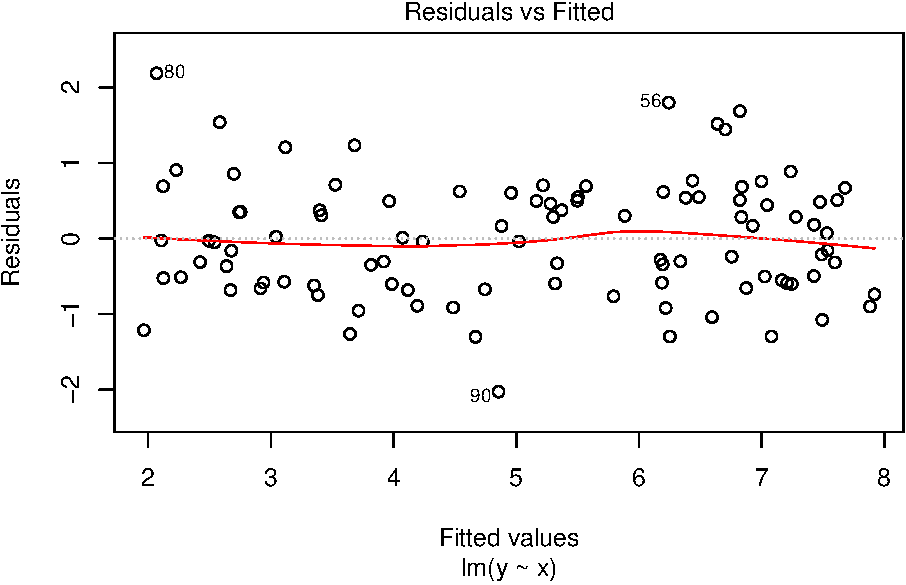
\includegraphics{./unnamed-chunk-26-1.pdf}
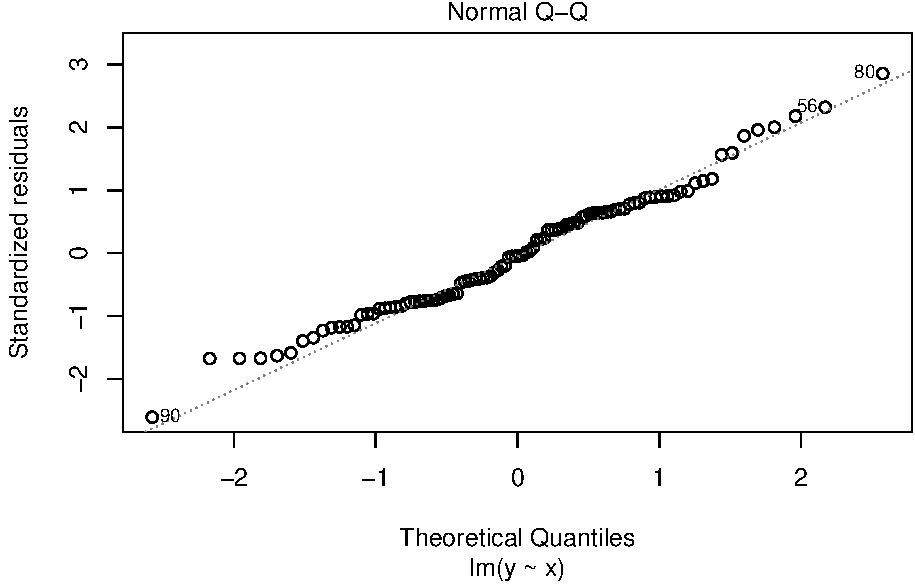
\includegraphics{./unnamed-chunk-26-2.pdf}
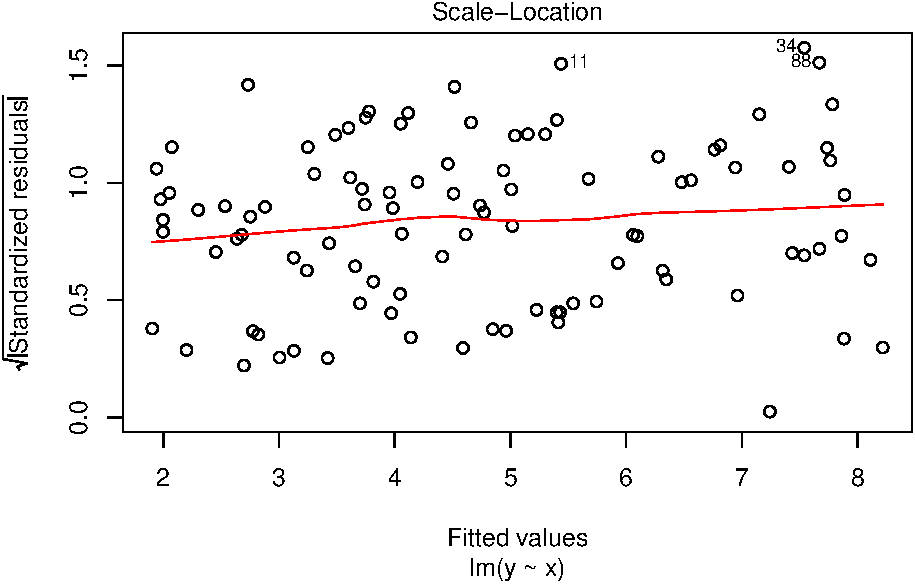
\includegraphics{./unnamed-chunk-26-3.pdf}
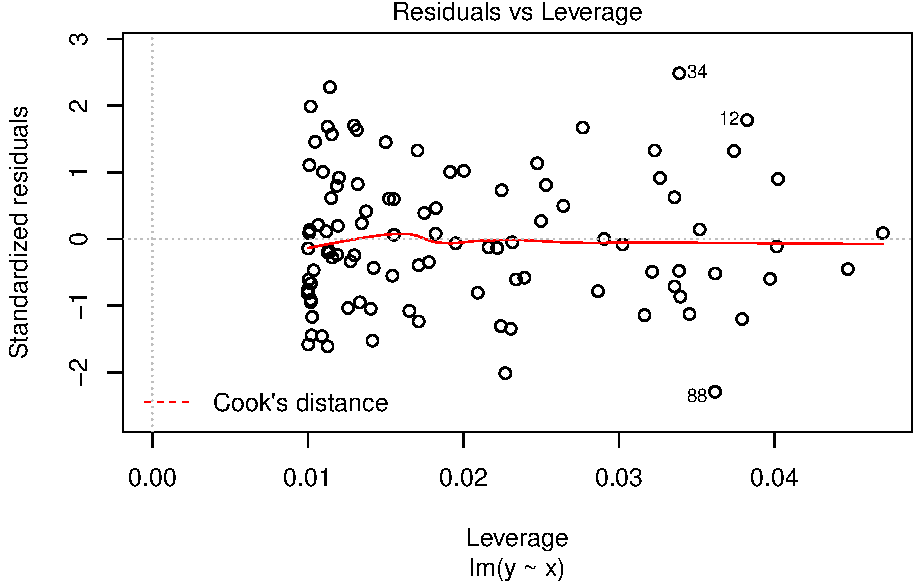
\includegraphics{./unnamed-chunk-26-4.pdf}

And that is basically it, at least for the basics. There is much more to
say about the \texttt{lm()} command, but that is for later.

\subsection{Making plots}\label{making-plots}

Where \texttt{R} truly shines is in making plots, diagrams, histograms,
etcetera. The first thing with data you want to do is to make a
scatterplot. With our previously defined \(x\) and \(y\) data this can
be easily done by:

\begin{Shaded}
\begin{Highlighting}[]
\KeywordTok{plot}\NormalTok{(x,y)}
\end{Highlighting}
\end{Shaded}

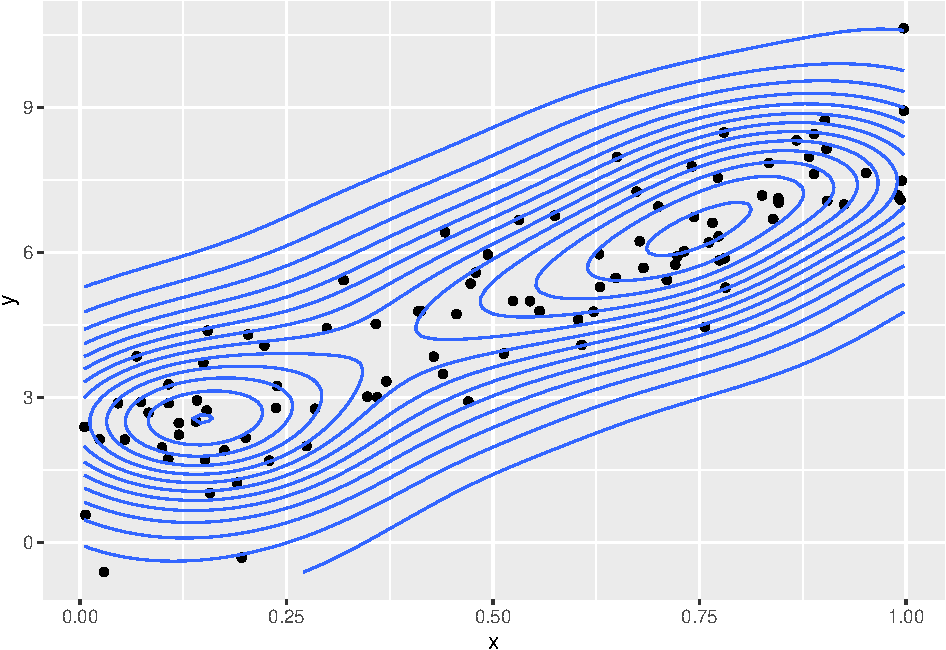
\includegraphics{./unnamed-chunk-27-1.pdf}

If you would like to create a histogram, just use \texttt{hist()} as

\begin{Shaded}
\begin{Highlighting}[]
\KeywordTok{hist}\NormalTok{(y)}
\end{Highlighting}
\end{Shaded}

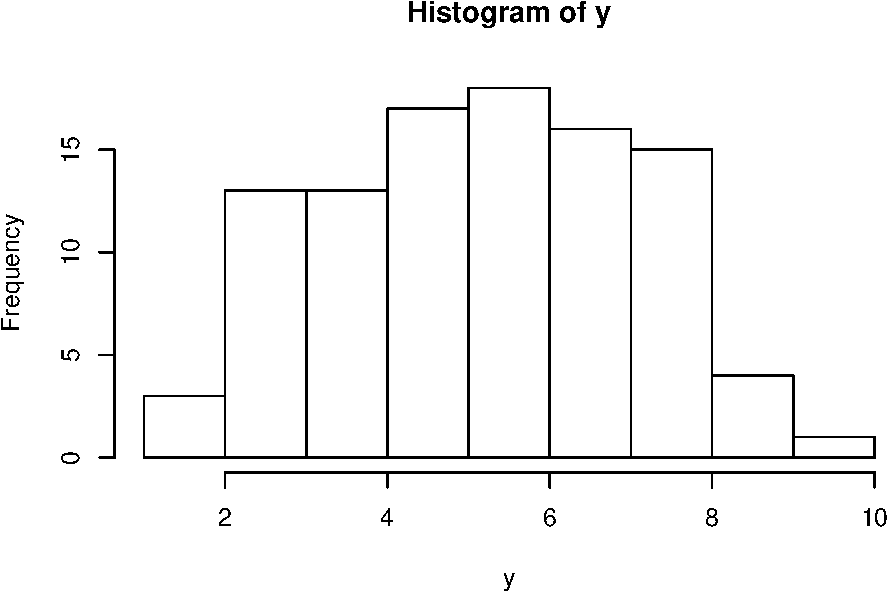
\includegraphics{./unnamed-chunk-28-1.pdf}

However, to go one step further you also make a plot of a dataframe. for
our df dataframe this is not very insightful, but let's add another
variable \(z\) uncorrelated with \(x\) and \(y\) and then plot the
dataframe (the \texttt{\$} indicate that \texttt{z} is a variable in
dataframe \texttt{df}).

\begin{Shaded}
\begin{Highlighting}[]
\NormalTok{df$z <-}\StringTok{ }\KeywordTok{runif}\NormalTok{(}\DecValTok{100}\NormalTok{, }\DecValTok{0}\NormalTok{,}\DecValTok{1}\NormalTok{)}
\KeywordTok{plot}\NormalTok{(df)}
\end{Highlighting}
\end{Shaded}

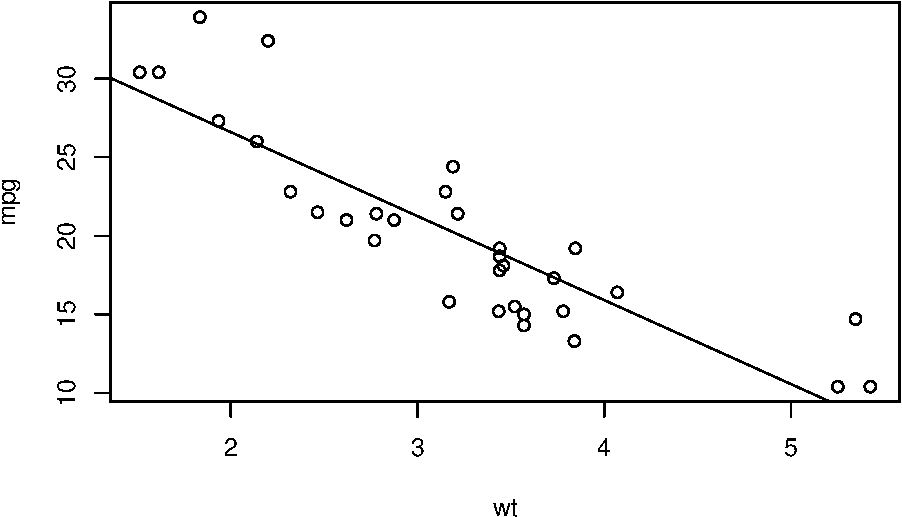
\includegraphics{./unnamed-chunk-29-1.pdf}

And luckily, this plot confirms what we expect. \(x\) are correlated
\(y\) by construction and \(z\) is not correlated with either \(x\) and
\(y\). These are all the so-called baseline plots. They are great (and
already highly customizable), but lately there has been a new kid on the
block called ggplot2. It goes to far to explain the details of ggplot2
(gg here stands for the grammar of graphics), but suffice to say that
ggplot2 works with building blocks, so that every piece of the figure
that you want (or can think of) can be constructed. Just as an example,
let's redo our scatterplot but now using ggplot2 and say we want to add
some density lines from our observations (just because we can). This can
be done in the following way

\begin{Shaded}
\begin{Highlighting}[]
\KeywordTok{ggplot}\NormalTok{(df, }\KeywordTok{aes}\NormalTok{(x,y))+}\KeywordTok{geom_point}\NormalTok{() +}\StringTok{ }\KeywordTok{geom_density2d}\NormalTok{()}
\end{Highlighting}
\end{Shaded}

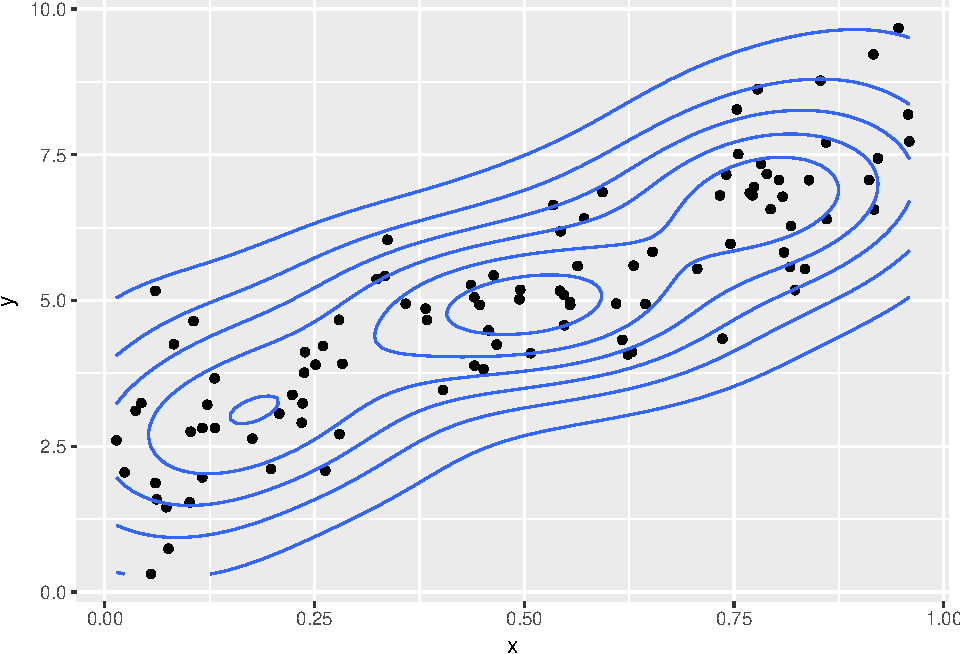
\includegraphics{./unnamed-chunk-30-1.pdf}

\subsection{Recap}\label{recap}

For the absolute beginner \texttt{R} is huge and daunting. You need to
learn by taking small steps and by practicing (a lot). Do not aim
immediately at big and complex projects but start small and at the
basics. You will then learn that you quickly make progress and at a
certain time even become efficienter than when using mouse driven tools
(clicking) as \texttt{Excel} or \texttt{SPSS}. In later chapters I dive
in to some more detailed topics, and hopefully the material provides you
with a background solid enough to understand and work with those topics
using \texttt{R}.

\section{Digression: Linear Regression and how to apply
it}\label{digression-linear-regression-and-how-to-apply-it}

\begin{Shaded}
\begin{Highlighting}[]
\KeywordTok{library}\NormalTok{(}\StringTok{"stargazer"}\NormalTok{)}
\end{Highlighting}
\end{Shaded}

In the social sciences (in fact, in all sciences) linear regressions
(also called OLS or ordinary least squares) or one of its relatives is
the most \emph{used} empirical research tool there is. Why? It is
relatively simple, computationally fast, easy to interpret and relies on
a relatively weak set of assumptions. Unfortunately, the assumptions
needed to be able to apply linear regression, are often not well
understood: both in the social sciences and beyond. Moreover, students
in the social sciences typically get little guidance in how to apply
linear regression in practice and how to interpret the results. Note
that this does not have anything to do with the specific software
students use, but more with that fact that regression techniques in a
wide number of situations (courses) are just not given (apart from
statistical or research methods courses). However, given the fact that
data becomes increasingly more available, knowing when to use regression
techniques, how to apply them and especially how to interpret and assess
them is now becoming an issue of paramount importance. Or, perhaps more
compelling, you need them to write your thesis.

In this chapter, I will first focus in section \ref{sec:theory} on the
\emph{essential} theory behind regression analysis. I really keep it to
the bare minimum. But if you understand these basics, I would argue that
you understand more than 75\% of the theorical background (the rest if
just nitty-gritty). Section \ref{sec:applications} will focus on
applications of linear regression, specification issues (how many
variables) and how to interpret the results.

\subsection{Theoretical background}\label{sec:theory}

This subsection first deals with the model (what are you trying to
explain), then about the three critical assumptions of (ordinary) least
squares, discusses subsequently typical situations when these
assumptions are violated, and finishes with a discussion about less
important stuff (on which, alas, quite some attention is given in
bachelor courses).

Before we start, I would like to make one important remark. In general,
statistical models can be used for (\emph{i}) finding
\textbf{statistical} relations, finding (\emph{ii}) \textbf{causal}
relations and for (\emph{iii}) \textbf{predicting}. All three uses
require the same assumptions, but have different focuses. In statistics,
generally the focus is on finding statistical relations, such as whether
the Dutch population is \emph{on average} taller then the German
population. In economics the focus is very much on finding causal
relations, so the need for explanatory power is not very large. Models
that do not explain much (where the \(R^2\)'s are low, say \(<\) 0.2)
are just as good as models that explain quite a lot, as long as the
least squares assumptions hold. In transportation science in general
(and other disciplines that deals with making large models) predictions
and thus explanatory power is key. Here it is now very important that
you perfectly understand what causes what as long as out-of-sample
predicting is good (say for predicting future commuting flows).

I usually have finding causal relations in mind when talking about least
squares (already difficult enough), but note again that the same least
squares assumptions, in some form or another, should hold when you want
to predict or want to find statistical relations.

\subsubsection{The model}\label{the-model}

Assume we are interested in the effect of the weight of a car on the
fuel efficiency of the car (measured in miles per gallon). We state the
following univariate regression model: \[
y_i = \alpha + \beta x_i + \epsilon_i,
\] where \(y\) denotes the fuel efficiency of the car, \(x\) denotes the
weight of the car and subscript \(i\) stands for the \(i\)-th
observation. \(\alpha\) and \(\beta\) are the parameters of the model
and they are \textbf{unknown} so they have to be \textbf{estimated}.
\(\epsilon\) is a so-called error term and denotes all the variation
that is not captured by our two variables (\(\alpha\) and \(\beta\)) and
our weight of the car variable \(x\).

The following observations are very important:

\begin{enumerate}
\def\labelenumi{\arabic{enumi}.}
\tightlist
\item
  What is on the left hand side of the \(=\) sign is what is to be
  explained (in this case miles per gallon). What is on the right hand
  side is what we use to explain \(y\); in this case being \(x\), the
  weight of the car.
\item
  The parameters \(\alpha\) en \(\beta\) constitute a \textbf{linear}
  relation between \(x\) and \(y\)
\item
  The parameter \(\alpha\) is the constant and in the univariate setting
  denotes where the linear relation crosses the \(y\)-axis.
\item
  \(\beta\) gives the impact of \(x\) on \(y\). Because it is a linear
  relation, the effect is simple. One unit change of \(x\) is associated
  with a \(\beta\) change of \(y\). In general, we can say that
  \(\beta\) is equal to the marginal effect
  (\(\frac{\partial y}{\partial x}\)). Moreover, in a univariate setting
  \(\beta\) denotes the slope of the relation between \(x\) and \(y\).
\item
  The regression error term \(\epsilon\) gives all variation that is not
  captured by our model, so \(y_i -(\alpha + \beta x_i) = \epsilon_i\).
  In this case, weight of the car most likely does not capture all
  variation in miles per gallon, so quite some variation is left in
  \(\epsilon\). Something else is captured as well by \(\epsilon\) and
  that is the measurement error of \(y\). So, if we have not measured
  miles per gallon precisely enough then that variation is captured as
  well by \(\epsilon\).
\end{enumerate}

Now, let's assume that we want to incorporate another variable (say the
number of cylinders, denoted by \(c\)), because we think that that
variable is very important as well in explaining miles per gallon. Then
we get the following \emph{multivariate} regression model: \[
y_i = \alpha + \beta_1 x_i + \beta_2 c_i + \epsilon_i,
\] where we now have two variables on the right hand side (\(x_i\) and
\(c_i\)) and three parameters (\(\alpha\), \(\beta_1\) and \(\beta_2\)).
In effect nothing changes with the intuition behind the model. Except
for the interpretation of the parameter \(\beta_1\) (and thus also
\(\beta_2\)). Parameter \(\beta_1\) now measures the impact of \(x\) on
\(y\) \emph{holding \(c\) constant}. So, multivariate regression models
is nothing more (and less) than controlling for other factors. And we
see later why that is very important.

\subsubsection{The least squares
assumptions}\label{the-least-squares-assumptions}

We are interested in the effect of the weight of the car on fuel
efficiency and,therefore, our \textbf{estimate} of \(\beta_1\) should be
very close to the \textbf{true} \(\beta_1\), especially when we have a
large number of observations. Regression is great and utterly brilliant
in finding this estimate, as long as the following three least squares
assumptions hold:

\begin{enumerate}
\def\labelenumi{\arabic{enumi}.}
\tightlist
\item
  There are no large outliers.
\item
  All left hand side (in this case \(y\)) and right side variables (in
  this case \(x\) and \(c\)) are \emph{i.i.d.}
\item
  For the error term the following must hold: \(E[\epsilon|X=x] = 0\).
\end{enumerate}

The first one is easy to understand. OLS is very sensitive to large
outliers in the dataset. It is therefore always good to look for
outliers and think whether they are \emph{real} observations or perhaps
typo's (in Excel or something). Do not throw outliers immediately away
but check whether they are correct.

The second is relatively easy to understand as well (but not that easy
to uphold in practice). \emph{i.i.d.} in this case stands for
independently and identically distributed. This basically means that the
observations in your dataset are independent from each other: in other
words, the observations should have been correctly \emph{sampled}.

The third looks the most horrible, and, to be quite honest, is so--both
in theory as in reality. This is also the assumption that is least well
understood; below, I will give some intuition what this assumptions
stands for. And especially in assessing whether regression output is
correct (is your estimate \emph{really} close to \(\beta_1\)) this
assumption is crucial.

\subsubsection{Possible violations and how to spot
them}\label{possible-violations-and-how-to-spot-them}

A violation of the first assumption is usually easy to spot. There is a
very strange outlier somewhere. But this also signifies the importance
of analysing \emph{descriptive statistics}, including means, maximums
and minimums, scatterplots and histograms.

Whether your data is not \emph{i.i.d.} can come because of a couple of
reasons. The most straightforward is getting your data via snowballing
(asking your friends and families using facebook to fill in a
questionnaire and to ask their friends and families to do so as well).
Usually, this means that you have a very specific sample and that the
estimate you get is not close to the true value for the whole
population. Observations might also be dependent upon each other,
because of unobserved factors. In our case, it might be that a type of
cars (American) are less fuel efficient than other cars (European).

Another typical violation of the \emph{i.i.d.} assumption is in
time-series, where what happened in the previous period might have a
large effect on the current period.

In general, however, violations of the \emph{i.i.d.} property are not
that devastating for your model as long as you are only interested in
finding the true \(\beta_1\): namely, it usually only affects the
precision of your estimate (the standard error) and not the estimate
itself. When this assumption is violated, we therefore say that the
estimate is \textbf{inefficient}. When you want to predict, however,
this assumption is crucial, as you would like your estimate to be
\emph{as precise} as possible.

When the third assumption is violated, we say that our estimate is
\textbf{biased}, in other words \textbf{wrong}: our parameter estimate
does not come close to the true parameter. And this happens more often
than not. So, what does \(E[\epsilon|X=x] = 0\) actually mean. Loosely
speaking, the parameters on the right hand side (in our case \(x\) and
\(c\)) on the one hand and the error term (\(\epsilon\)) on the other
hand are not allowed to be correlated. There are several ways how this
might happen, from which the following are in our case the most
relevant:

\begin{enumerate}
\def\labelenumi{\arabic{enumi})}
\item
  Reverse causality: \(x\) impacts \(y\), but \(y\) might impact \(x\)
  as well. This is the classical chicken and egg problem. Do firms
  perform better because of good management, or do good managers go to
  the better performing firms?
\item
  Unobserved heterogeneity bias: there are factors that are not in the
  model but influence both \(x\) and \(y\). For example, if american
  cars have both an influence on fuel efficiency and weight of the cars
  then the estimate that we find is not close to the true value of
  \(\beta_1\).
\item
  Misspecification: we assume that our model is linear, but it actually
  is not. Then, again, our estimate that we find is not close to the
  true value of \(\beta_1\).
\end{enumerate}

There are other sources of violations, but in this case, these are the
most important ones. Reverse causality is usually hard to correct for,
but unobserved heterogeneity bias is luckily easier. Namely, we add
\emph{relevant} control variables (as we did with \(c\)). In this case
we can \emph{minimize} possible unobserved heterogeity bias.
Misspefications are in general as well relatively easy to correct for.
From our descriptive statistics and scatterplot we usually can infer the
relation between \(x\) and \(y\) and control for possible nonlinearities
by using (natural) logarithms and squared terms.

As a sidenote, natural logarithms are the ones most used for various
reasons not discussed here. If we take the logarithm of both sides then
for our univariate regression we get: \[
\ln(y_i) = \alpha + \beta \ln(x_i) + \epsilon_i,
\] and all the aforementioned rules and assumptions still apply. But
there is something peculiar to this regression. Namely, if we are
interested in the marginal effect (\(\frac{\partial y}{\partial x}\)),
we get the following: \[
\frac{\partial y}{\partial x} = \frac{\partial e^{\ln(y_t)}}{\partial x} = \frac{\partial e^{(\alpha + \beta \ln(x_i) + \epsilon_i)}}{\partial x} = \frac{\beta}{x}e^{(\alpha + \beta \ln(x_i) + \epsilon_i)} = \frac{\beta}{x}y, 
\] In other words: \[
\beta = \frac{\partial y}{\partial x} \frac{x}{y}
\] which is simply the \textbf{elasticity} between \(x\) and \(y\). So,
if there are logarithms on both the left and right hand side then the
parameters (the \(\beta\)'s) denotes elasticities.

\subsubsection{Normality, heteroskedasticity and
multicollinearity}\label{normality-heteroskedasticity-and-multicollinearity}

Until now, we have not discussed the concepts normality,
heteroskedasticity and multicollinearity. That is simply because they
are not that relevant (as long as we have enough observations, typically
above 40). The validity of OLS hinges just upon the three assumptions
mentioned above (and they are already difficult enough). In fact, if the
three assumptions are satisfied, then, as an \textbf{outcome}, the
parameters (\(\beta\)) are normally distributed. It goes to far to
explain why (the theorems required for this are deeply fundamental to
statistics), but in any case, normality is \textbf{not} a core OLS
assumption. It would be nice if both \(y\) and \(x\) are normally
distributed because then the standard errors are minimized, but again,
whether the estimate of \(\beta\) you find is correct or not (biased or
unbiased) does not depend on normality \textbf{assumptions}.

Heteroskedasticy (in other words your standard errors are not constant)
as well leads to quite some confusion. In general heteroskedasticity
only leads to inefficient estimates (so only affects the standard
errors). Nothing more, nothing less. And there are corrections for that
(robust standard errors in \texttt{Stata} and similar procedures in
\texttt{R}), so that nobody needs to care anymore about
heteroskedasticity.

Finally, there is multicollinearity. And this comes in two flavours:
perfect and imperfect multicollinearity. Perfect multicollinearity
occurs, e.g., when your model contains two identical variables. Then,
OLS can not decide which one to use and usually one of the variables is
dropped, or your computer program gives an error (\emph{computer says
no}).

Imperfect multicollinearity occurs when two variables are highly (but
not perfectly) correlated. This occurs less often than one may think.
Variables that are highly correlated (say \(age\) and \(age^2\)) can be
perfectly incorporated in a model. Only when the correlation becomes
very high (say above 95\% or even higher) then something strange
happens: the standard errors get very large. Why? That is because of the
definition mentioned above. Parameter \(\beta_1\) measures the impact of
\(x\) on \(y\) \emph{holding \(c\) constant}. But if \(x\) and \(c\) are
very highly correlated and you control for \(c\), then not much
variation is left over for \(x\). So, \(c\) actually removes the
variation \emph{within} the variable \(x\). This always happens, and
there is a trade-off between adding more variables and leaving enough
variation (note that there is always correlation between variables), but
usually it all goes fine. Good judgement and sound thinking typically
helps more than strange statistics (say VIF?).

\subsection{Applications of linear regression}\label{sec:applications}

This section gives an application of regression analysis. Assume we are
still interested in the effect of the weight of a car on the fuel
efficiency of the car (measures in miles per gallon). We have found a
dataset (internal in \texttt{R}), so the first thing we have to do is
look at the descriptives of the dataset.

\subsubsection{Descriptives}\label{descriptives}

The build-in dataset \texttt{mtcars} has, besides several other
variables, information on weight of a car (in 1000 lbs or in about 450
kilos) and miles per gallon. With the following command \texttt{head()}
we can look at the first 6 observations.

\begin{Shaded}
\begin{Highlighting}[]
\KeywordTok{head}\NormalTok{(mtcars)}
\end{Highlighting}
\end{Shaded}

\begin{verbatim}
##                    mpg cyl disp  hp drat    wt  qsec vs am gear carb
## Mazda RX4         21.0   6  160 110 3.90 2.620 16.46  0  1    4    4
## Mazda RX4 Wag     21.0   6  160 110 3.90 2.875 17.02  0  1    4    4
## Datsun 710        22.8   4  108  93 3.85 2.320 18.61  1  1    4    1
## Hornet 4 Drive    21.4   6  258 110 3.08 3.215 19.44  1  0    3    1
## Hornet Sportabout 18.7   8  360 175 3.15 3.440 17.02  0  0    3    2
## Valiant           18.1   6  225 105 2.76 3.460 20.22  1  0    3    1
\end{verbatim}

Again, we are interested in the relation weight of a car (the variable
\texttt{wt}) and miles per gallon (the variable \texttt{mpg}). Note,
that in his case \texttt{mpg} is the first column and \texttt{wt} is the
sixth column. (The column with car names above is not a real variable,
but are the row names). Recall that the command \texttt{c()} combines
stuff, so we can look at the summary statistics of the variables we are
only interested in by:

\begin{Shaded}
\begin{Highlighting}[]
\KeywordTok{summary}\NormalTok{(mtcars[,}\KeywordTok{c}\NormalTok{(}\DecValTok{1}\NormalTok{,}\DecValTok{6}\NormalTok{)])}
\end{Highlighting}
\end{Shaded}

\begin{verbatim}
##       mpg              wt       
##  Min.   :10.40   Min.   :1.513  
##  1st Qu.:15.43   1st Qu.:2.581  
##  Median :19.20   Median :3.325  
##  Mean   :20.09   Mean   :3.217  
##  3rd Qu.:22.80   3rd Qu.:3.610  
##  Max.   :33.90   Max.   :5.424
\end{verbatim}

There does not seem to be anything out of the ordinary here, but to be
sure, we construct a scatterplot between weight of the car and miles per
gallon.

\begin{Shaded}
\begin{Highlighting}[]
\KeywordTok{plot}\NormalTok{(mpg~wt, mtcars)}
\end{Highlighting}
\end{Shaded}

\begin{figure}[htbp]
\centering
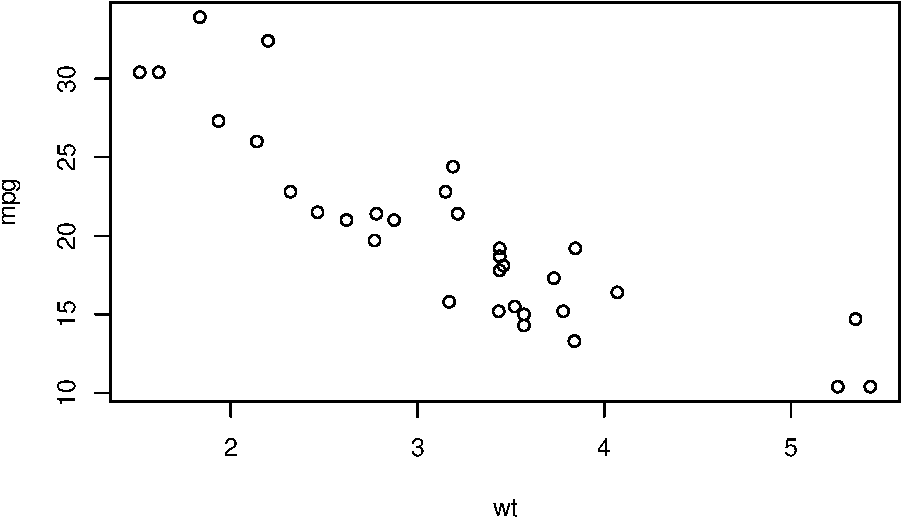
\includegraphics{./unnamed-chunk-34-1.pdf}
\caption{\label{fig:unnamed-chunk-34}A scatterplog between miles per gallon
and car weight.}
\end{figure}

So, there do not seem to be many outliers here. Moreover, as we would
expect, there seems to be a downward sloping relation between weight of
the car and miles per gallon (hopefully you agree, that this makes
sense). To \textbf{quantify} this relation, the next subsection will
perform a least squares estimation.

\subsubsection{Baseline model}\label{baseline-model}

So, if we are only interested in the relation between weight of a car
(the variable \texttt{wt}) and miles per gallon, we can easily perform
the following regression (recall again that the command \texttt{lm()}
performs a least squares estimation and that \texttt{\textless{}-}
denotes an assignment to a variable:

\begin{Shaded}
\begin{Highlighting}[]
\NormalTok{baselinemodel <-}\StringTok{ }\KeywordTok{lm}\NormalTok{(mpg~wt, mtcars)}
\KeywordTok{summary}\NormalTok{(baselinemodel)}
\end{Highlighting}
\end{Shaded}

\begin{verbatim}
## 
## Call:
## lm(formula = mpg ~ wt, data = mtcars)
## 
## Residuals:
##     Min      1Q  Median      3Q     Max 
## -4.5432 -2.3647 -0.1252  1.4096  6.8727 
## 
## Coefficients:
##             Estimate Std. Error t value Pr(>|t|)    
## (Intercept)  37.2851     1.8776  19.858  < 2e-16 ***
## wt           -5.3445     0.5591  -9.559 1.29e-10 ***
## ---
## Signif. codes:  0 '***' 0.001 '**' 0.01 '*' 0.05 '.' 0.1 ' ' 1
## 
## Residual standard error: 3.046 on 30 degrees of freedom
## Multiple R-squared:  0.7528, Adjusted R-squared:  0.7446 
## F-statistic: 91.38 on 1 and 30 DF,  p-value: 1.294e-10
\end{verbatim}

At this point it is good to stop and see what we have got. We have the
formula call (we know this one), some stuff about the residuals, stuff
about the coefficients (most important for us), and some diagnostics
(including the notorious \(R^2\)). We zoom in on the results about the
coefficients. We have an estimation of the intercept (our \(\alpha\) of
above) and of \texttt{wt} (our \(\beta\) of above). For both, we have as
well a standard error, a \(t\)-value, a probability and a bunch of
stars. What do they all mean again? We focus on \texttt{wt} here
(typically we are less interested in the constant or intercept).

The estimate is easy; that is \(\beta\) or the marginal effect of \(x\)
on \(y\). So, increasing \(x\) with 1 (or with a 1000 lbs) decreases the
miles per gallon with 5.3445 (which is quite a lot).

The standard error denotes the \emph{precision} of the estimate. As a
rule of thumb: you know with 95\% centainty that the true value of
\(\beta\) lies within the interval {[}estimate \(- 2 \times\) standard
error, estimate \(+ 2 \times\) standard error{]}. The standard error is
very important and is used to \textbf{test} possible values of the
parameter. One of the most important tests is whether \(\beta=0\). Why?
Because, if \(\beta=0\) then the variable \texttt{wt} does nothing on
\texttt{mpg}. This specific test is always denoted by the \(t\)-value,
its associated probability and the corresponding star thingies. In this
case, the \(t\)-value is high in an absolute sense, so it is \emph{very}
improbable that the estimate could be zero (somehting like a probability
of 0.0000000001 which is small indeed), and the stars neatly indicate
that this probability (of \(\beta=0\)) is smaller than 0.001.

One nice trick is to plot the regression line in the scatterplot above.
One can do so by the command \texttt{abline()} or:

\begin{Shaded}
\begin{Highlighting}[]
\KeywordTok{plot}\NormalTok{(mpg~wt, mtcars)}
\KeywordTok{abline}\NormalTok{(}\KeywordTok{lm}\NormalTok{(mpg~wt, mtcars))}
\end{Highlighting}
\end{Shaded}

\begin{figure}[htbp]
\centering
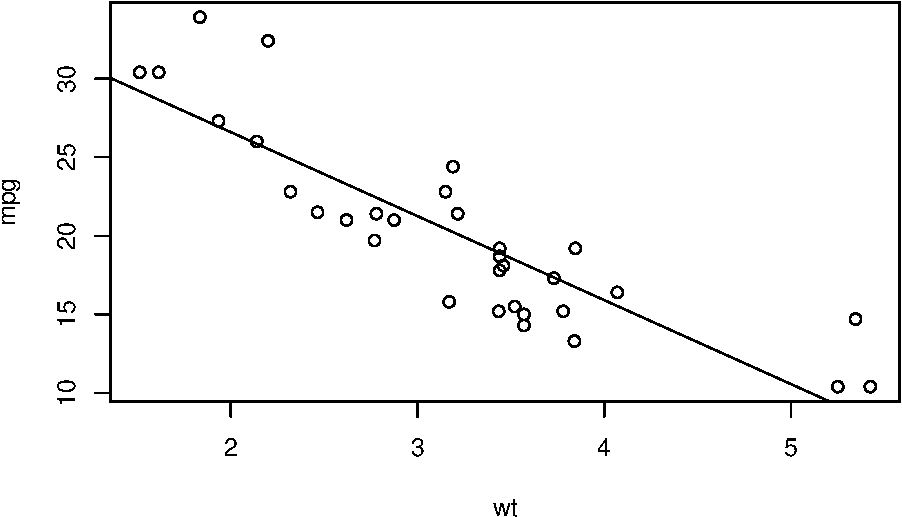
\includegraphics{./unnamed-chunk-36-1.pdf}
\caption{\label{fig:unnamed-chunk-36}A scatterplog between miles per gallon
and car weight with regression line.}
\end{figure}

\subsubsection{Specificion issues}\label{specificion-issues}

I can imagine that you are not very satisfied yet with the analysis.
First of all, the relation between \texttt{mpg} and \texttt{wt} might be
nonlinear and, secondly, you would like to include additional variables.
First we look at the possible nonlinearity in the regression relation
(note that we can use the regression formula as before, but that we can
specify logarithmic relations by \texttt{log()}):

\begin{Shaded}
\begin{Highlighting}[]
\NormalTok{logmodel <-}\StringTok{ }\KeywordTok{lm}\NormalTok{(}\KeywordTok{log}\NormalTok{(mpg)~}\KeywordTok{log}\NormalTok{(wt), mtcars)}
\KeywordTok{summary}\NormalTok{(logmodel)}
\end{Highlighting}
\end{Shaded}

\begin{verbatim}
## 
## Call:
## lm(formula = log(mpg) ~ log(wt), data = mtcars)
## 
## Residuals:
##      Min       1Q   Median       3Q      Max 
## -0.18141 -0.10681 -0.02125  0.08109  0.26930 
## 
## Coefficients:
##             Estimate Std. Error t value Pr(>|t|)    
## (Intercept)  3.90181    0.08790   44.39  < 2e-16 ***
## log(wt)     -0.84182    0.07549  -11.15 3.41e-12 ***
## ---
## Signif. codes:  0 '***' 0.001 '**' 0.01 '*' 0.05 '.' 0.1 ' ' 1
## 
## Residual standard error: 0.1334 on 30 degrees of freedom
## Multiple R-squared:  0.8056, Adjusted R-squared:  0.7992 
## F-statistic: 124.4 on 1 and 30 DF,  p-value: 3.406e-12
\end{verbatim}

We have now the same type of output as before, but I would like to focus
on two things here. First, the \(R^2\) has gone up and that is what you
typically get in the social sciences. Logarithmically transformed
variables usually \textbf{fit} better. Secondly, the interpretation of
the estimate now differs. It has become an elasticity with size
\(-0.84\), which is quite high again. If the car doubles in weights, the
fuel efficiency of the car goes down by 84\%!

Secondly, you might want to include other variables, such as being a
foreing car (opposite to a car from the US) (\texttt{vs}), the number of
cylinders (\texttt{cyl}), the gross horsepower (\texttt{hp}) and how
quick the car does over a quarter of a mile (\texttt{qsec}). Again, we
are not interested in these additional variables or whether they crank
up the \(R^2\). The only thing we are interested is in whether the
coefficient of \texttt{log(wt)} changes.

\begin{Shaded}
\begin{Highlighting}[]
\NormalTok{extendedmodel <-}\StringTok{ }\KeywordTok{lm}\NormalTok{(}\KeywordTok{log}\NormalTok{(mpg)~}\KeywordTok{log}\NormalTok{(wt)+vs+cyl +}\StringTok{ }\NormalTok{hp +}\StringTok{ }\NormalTok{qsec, mtcars)}
\KeywordTok{summary}\NormalTok{(extendedmodel)}
\end{Highlighting}
\end{Shaded}

\begin{verbatim}
## 
## Call:
## lm(formula = log(mpg) ~ log(wt) + vs + cyl + hp + qsec, data = mtcars)
## 
## Residuals:
##       Min        1Q    Median        3Q       Max 
## -0.201746 -0.065242 -0.009506  0.079809  0.205166 
## 
## Coefficients:
##               Estimate Std. Error t value Pr(>|t|)    
## (Intercept)  3.5280554  0.4610947   7.651 4.04e-08 ***
## log(wt)     -0.6514583  0.1509786  -4.315 0.000205 ***
## vs          -0.0149215  0.0863277  -0.173 0.864111    
## cyl         -0.0160253  0.0314486  -0.510 0.614651    
## hp          -0.0007670  0.0006861  -1.118 0.273786    
## qsec         0.0212017  0.0267153   0.794 0.434603    
## ---
## Signif. codes:  0 '***' 0.001 '**' 0.01 '*' 0.05 '.' 0.1 ' ' 1
## 
## Residual standard error: 0.1121 on 26 degrees of freedom
## Multiple R-squared:  0.8811, Adjusted R-squared:  0.8582 
## F-statistic: 38.53 on 5 and 26 DF,  p-value: 3.227e-11
\end{verbatim}

Clearly, the coefficient of \texttt{log(wt)} changes with the inclusion
of additional variables. So there was unobserved heterogeneity bias in
our baseline model (and most likely there still is in our extended
model), even though the addional variables are not siginficant.

\subsubsection{Reporting}\label{reporting}

Hopefully you agree that the regression output of above looks
\textbf{horrible} and that you do not need all these statistics and
stuff. Therefore, you need to construct your own table for presentation
format. The minimum what should be in these tables are the coefficient
names, the estimates, the standard errors (and the stars would be nice
as well), the \(R^2\) and the number of observations used.

Unfortunately, creating tables of your own is a pain in the \ldots{}
Luckily, within \texttt{R} (and by the way in programs as \texttt{Stata}
as well) you can do this automatically! In \texttt{R} there are several
packages one can use. I prefer the package Stargazer and after using
this package we get the following outcome for our logarithmic
specification:\footnote{To get nice tables directly into \texttt{Word},
  you need something else (as you can imagine, because \texttt{Word} is
  not scriptable). With Stargazer you should give the command as such
  \texttt{stargazer(logmodel,\ extendedmodel,\ out\ =\ "table1.txt",omit.stat\ =\ c("rsq",\ "f"))}
  and thereafter you can read in and edit the table
  \texttt{table1.txt}in \texttt{Word}.}

\begin{Shaded}
\begin{Highlighting}[]
\KeywordTok{stargazer}\NormalTok{(logmodel, extendedmodel, }\DataTypeTok{header=}\OtherTok{FALSE}\NormalTok{, }\DataTypeTok{type =} \StringTok{"html"}\NormalTok{, }\DataTypeTok{omit.stat =} \KeywordTok{c}\NormalTok{(}\StringTok{"rsq"}\NormalTok{, }\StringTok{"f"}\NormalTok{))}
\end{Highlighting}
\end{Shaded}

Dependent variable:

log(mpg)

(1)

(2)

log(wt)

-0.842***

-0.651***

(0.075)

(0.151)

vs

-0.015

(0.086)

cyl

-0.016

(0.031)

hp

-0.001

(0.001)

qsec

0.021

(0.027)

Constant

3.902***

3.528***

(0.088)

(0.461)

Observations

32

32

Adjusted R2

0.799

0.858

Residual Std. Error

0.133 (df = 30)

0.112 (df = 26)

Note:

\emph{p\textless{}0.1; \textbf{p\textless{}0.05; }}p\textless{}0.01

Note that we now display both specifications, the first the univariate
case and the second the multivariate case. This is now typically done in
social science research. You start with a baseline and then add
variables to check whether the variable of interest remains robust.

\subsubsection{Internal validation}\label{internal-validation}

So, after done all modeling exercitions you are not done! Now, it is
time to validate your results internally. Can you be confident of your
results? Or is the parameter that you have found still suspect of
possible biases. Here again come the three least squares assumptions:

\begin{enumerate}
\def\labelenumi{\arabic{enumi}.}
\item
  No large outliers: we have checked that with our descriptive
  statistics and our scatterplot and it seems that this assumption is
  met.
\item
  Both miles per gallon and car weight should be \emph{i.i.d.}. We can
  reasonably assume that the sampling has been done correctly.
\item
  The following condition should hold: \(E[\epsilon|X=x] = 0\). This one
  is dubious. Probably there is no reverse causality (difficult to image
  that miles per gallon would influence car weight), but most likely
  there are other factors that impact car weight and miles per gallon
  which are omitted (where is the car build, what is the car brand,
  etcetera.). One possible strategy here is to add additional variables
  until the parameter of interest remains robust (does not change
  anymore).
\end{enumerate}

Note that the number of observations in this case is only 32, so whether
our standard errors are automatically normally distributed is highly
questionable, but for the sake of the exposition (and the fact that
small sample statistics are very complex) we leave it just with this
observation.

\section{\texorpdfstring{Network analysis with
\texttt{R}}{Network analysis with R}}\label{network-analysis-with-r}

\begin{Shaded}
\begin{Highlighting}[]
\KeywordTok{library}\NormalTok{(}\StringTok{"igraph"}\NormalTok{)}
\KeywordTok{library}\NormalTok{(}\StringTok{"igraphdata"}\NormalTok{)}
\KeywordTok{library}\NormalTok{(}\StringTok{"networkD3"}\NormalTok{)}
\end{Highlighting}
\end{Shaded}

\subsection{Introduction}\label{introduction-1}

Network analysis is huge and applied in many disciplines, ranging from
mathematics to sociology. In \texttt{R} there are many packages
available. We will use the \texttt{igraph} package, which seems to be
the most encompassing.\footnote{Obviously I want to provide a
  self-contained manual, however, there are as well some pretty good and
  more extensive tutorials on internet: e.g., the one over
  \href{http://kateto.net/networks-r-igraph/}{here}.} The next sections
first starts with creating networks on our own (from scratch), then I
show how to make structured networks and finally we create networks from
data. Thereafter, I say something about creating interactive networks
(those cool things, you sometimes see on internet). The last section
deals with calculating network characteristics.

\subsection{Creating networks}\label{creating-networks}

There are various ways to create a network: one can it oneself, one can
create a structured network, and one can read a network from file or the
internet. (The latter is typically done with very large and dynamics
network data.)

\subsubsection{Creating network
yourself}\label{creating-network-yourself}

First of all, I will show how to create a network ``by hand''. We first
start with an undirected network. Suppose we have a network with four
nodes (named 1,2, 3 and, you guessed it, 4). Then we can create a graph
called \texttt{g\_4} by:

\begin{Shaded}
\begin{Highlighting}[]
\NormalTok{g_4 <-}\StringTok{ }\KeywordTok{graph} \NormalTok{(}\DataTypeTok{edges =} \KeywordTok{c}\NormalTok{(}\DecValTok{1}\NormalTok{,}\DecValTok{2}\NormalTok{,}\DecValTok{2}\NormalTok{,}\DecValTok{3}\NormalTok{,}\DecValTok{3}\NormalTok{,}\DecValTok{4}\NormalTok{, }\DecValTok{4}\NormalTok{,}\DecValTok{1}\NormalTok{), }\DataTypeTok{n =} \DecValTok{4}\NormalTok{, }\DataTypeTok{directed =} \OtherTok{FALSE}\NormalTok{)}
\end{Highlighting}
\end{Shaded}

Let us have a look at \texttt{g\_4}

\begin{Shaded}
\begin{Highlighting}[]
\NormalTok{g_4}
\end{Highlighting}
\end{Shaded}

\begin{verbatim}
## IGRAPH 803f1cd U--- 4 4 -- 
## + edges from 803f1cd:
## [1] 1--2 2--3 3--4 1--4
\end{verbatim}

So, \texttt{g\_4} is an igraph sort of object which has four edges
\texttt{1-\/-2\ 2-\/-3\ 3-\/-4\ 1-\/-4}. Note that these coincide with
\texttt{c(1,2,2,3,3,4,\ 4,1)}, so an edge is always formed by two
components (they do not have to be numbers). Now plotting \texttt{g\_4}
leads to:

\begin{Shaded}
\begin{Highlighting}[]
\KeywordTok{plot}\NormalTok{(g_4)}
\end{Highlighting}
\end{Shaded}

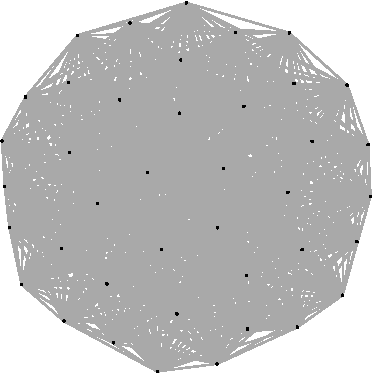
\includegraphics{ResearchTools_files/figure-latex/unnamed-chunk-43-1.pdf}

The connectivity matrix of the network can be directly given by:

\begin{Shaded}
\begin{Highlighting}[]
\NormalTok{g_4[]}
\end{Highlighting}
\end{Shaded}

\begin{verbatim}
## 4 x 4 sparse Matrix of class "dgCMatrix"
##             
## [1,] . 1 . 1
## [2,] 1 . 1 .
## [3,] . 1 . 1
## [4,] 1 . 1 .
\end{verbatim}

Now, for more directed graphs we need to set \texttt{directed\ =\ TRUE}.

\begin{Shaded}
\begin{Highlighting}[]
\NormalTok{g_4 <-}\StringTok{ }\KeywordTok{graph} \NormalTok{(}\DataTypeTok{edges =} \KeywordTok{c}\NormalTok{(}\DecValTok{1}\NormalTok{,}\DecValTok{2}\NormalTok{,}\DecValTok{2}\NormalTok{,}\DecValTok{3}\NormalTok{,}\DecValTok{3}\NormalTok{,}\DecValTok{4}\NormalTok{, }\DecValTok{4}\NormalTok{,}\DecValTok{1}\NormalTok{), }\DataTypeTok{n =} \DecValTok{4}\NormalTok{, }\DataTypeTok{directed =} \OtherTok{TRUE}\NormalTok{)}
\end{Highlighting}
\end{Shaded}

with as plot

\begin{Shaded}
\begin{Highlighting}[]
\KeywordTok{plot}\NormalTok{(g_4)}
\end{Highlighting}
\end{Shaded}

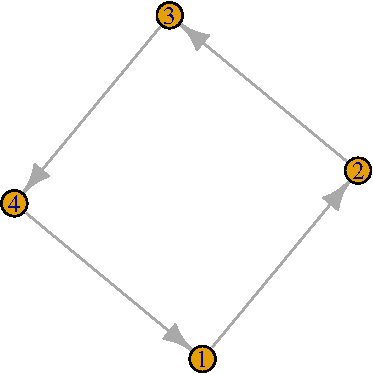
\includegraphics{ResearchTools_files/figure-latex/unnamed-chunk-46-1.pdf}

Graphs may also be generated by using \texttt{-}, \texttt{-+} and
\texttt{+-+}, in combination with the command
\texttt{graph\_from\_literal}. For example:

\begin{Shaded}
\begin{Highlighting}[]
\NormalTok{g_directed <-}\StringTok{ }\KeywordTok{graph_from_literal}\NormalTok{(A-+B, B +-+}\StringTok{ }\NormalTok{C, C+-A)}
\KeywordTok{plot}\NormalTok{(g_directed)}
\end{Highlighting}
\end{Shaded}

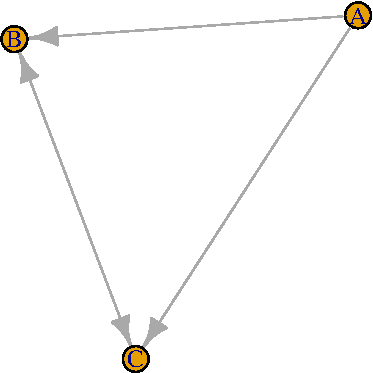
\includegraphics{ResearchTools_files/figure-latex/unnamed-chunk-47-1.pdf}

Finally, we can influence the color and sizes (amongst others) of all
the elements of the network, so:

\begin{Shaded}
\begin{Highlighting}[]
\KeywordTok{plot}\NormalTok{(g_directed, }\DataTypeTok{edge.arrow.size=}\DecValTok{2}\NormalTok{,}\DataTypeTok{vertex.size =} \DecValTok{50}\NormalTok{, }\DataTypeTok{vertex.color =} \StringTok{"blue"} \NormalTok{)}
\end{Highlighting}
\end{Shaded}

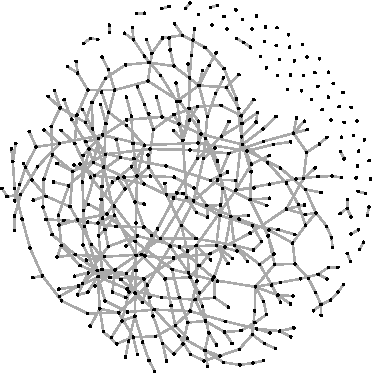
\includegraphics{ResearchTools_files/figure-latex/unnamed-chunk-48-1.pdf}

However, this way of creating of networks is not very efficient. We
therefore offer some other ways as well, starting with created directly
(well-structured networks).

\subsubsection{Structured networks}\label{structured-networks}

With the package \texttt{igraph} it is rather straighforward to create
structured networks. Let's start with an empty network. We therefore use
the command \texttt{make\_empty\_graph(500} in order to create 500 nodes
and no links.

\begin{Shaded}
\begin{Highlighting}[]
\NormalTok{g_empty <-}\StringTok{ }\KeywordTok{make_empty_graph}\NormalTok{(}\DecValTok{500}\NormalTok{)}
\KeywordTok{plot}\NormalTok{(g_empty, }\DataTypeTok{vertex.label=} \OtherTok{NA}\NormalTok{, }\DataTypeTok{edge.arrow.size=}\FloatTok{0.02}\NormalTok{,}\DataTypeTok{vertex.size =} \FloatTok{0.5}\NormalTok{)}
\end{Highlighting}
\end{Shaded}

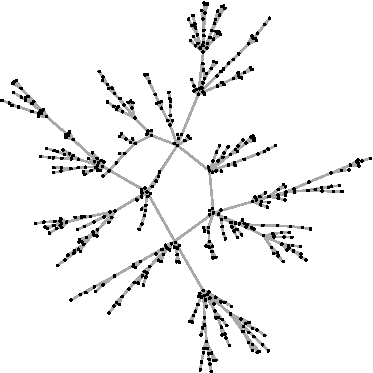
\includegraphics{ResearchTools_files/figure-latex/unnamed-chunk-49-1.pdf}

The other extreme is obviously the fully connected network. With the
command \texttt{make\_full\_graph(40)} we can create a fully connected
network between 40 nodes. (Please do not do 500 nodes; it takes a long
time to create that network (with \(500 \times 500 - 500\) links)).

\begin{Shaded}
\begin{Highlighting}[]
\NormalTok{g_full <-}\StringTok{ }\KeywordTok{make_full_graph}\NormalTok{(}\DecValTok{40}\NormalTok{)}
\KeywordTok{plot}\NormalTok{(g_full, }\DataTypeTok{vertex.label=} \OtherTok{NA}\NormalTok{, }\DataTypeTok{edge.arrow.size=}\FloatTok{0.02}\NormalTok{,}\DataTypeTok{vertex.size =} \FloatTok{0.5}\NormalTok{)}
\end{Highlighting}
\end{Shaded}

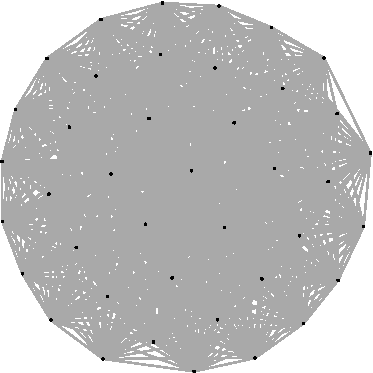
\includegraphics{ResearchTools_files/figure-latex/unnamed-chunk-50-1.pdf}

The \texttt{make\_star(500)} command create a star network (or a
hub-and-spoke network) with 500 nodes.

\begin{Shaded}
\begin{Highlighting}[]
\NormalTok{g_star <-}\StringTok{ }\KeywordTok{make_star}\NormalTok{(}\DecValTok{500}\NormalTok{)}
\KeywordTok{plot}\NormalTok{(g_star, }\DataTypeTok{vertex.label=} \OtherTok{NA}\NormalTok{, }\DataTypeTok{edge.arrow.size=}\FloatTok{0.02}\NormalTok{,}\DataTypeTok{vertex.size =} \FloatTok{0.5}\NormalTok{)}
\end{Highlighting}
\end{Shaded}

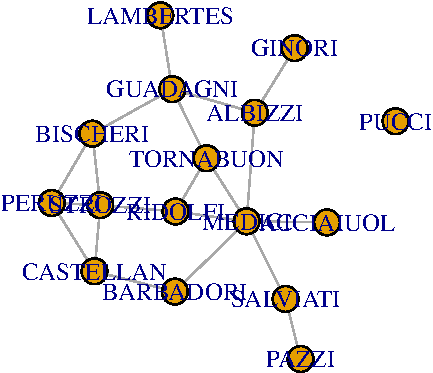
\includegraphics{ResearchTools_files/figure-latex/unnamed-chunk-51-1.pdf}

With the \texttt{make\_tree(500,\ children\ =\ 3,\ mode="undirected}
command, we create an undirected hierarchical tree with each time tree
children

\begin{Shaded}
\begin{Highlighting}[]
\NormalTok{g_tree <-}\StringTok{ }\KeywordTok{make_tree}\NormalTok{(}\DecValTok{500}\NormalTok{, }\DataTypeTok{children =} \DecValTok{3}\NormalTok{, }\DataTypeTok{mode =} \StringTok{"undirected"}\NormalTok{)}
\KeywordTok{plot}\NormalTok{(g_tree, }\DataTypeTok{vertex.label=} \OtherTok{NA}\NormalTok{, }\DataTypeTok{edge.arrow.size=}\FloatTok{0.02}\NormalTok{,}\DataTypeTok{vertex.size =} \FloatTok{0.5}\NormalTok{)}
\end{Highlighting}
\end{Shaded}

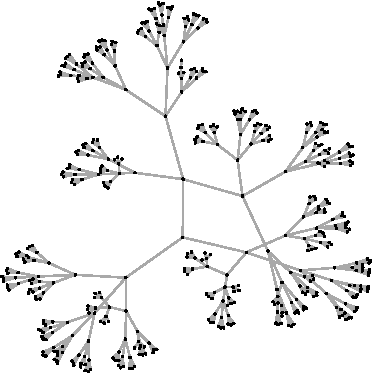
\includegraphics{ResearchTools_files/figure-latex/unnamed-chunk-52-1.pdf}

And the \texttt{graph.ring(500)} creates a ring (or line) structure
where each node is connected to two other nodes in a sequential way

\begin{Shaded}
\begin{Highlighting}[]
\NormalTok{g_ring <-}\StringTok{ }\KeywordTok{graph.ring}\NormalTok{(}\DecValTok{500}\NormalTok{)}
\KeywordTok{plot}\NormalTok{(g_ring, }\DataTypeTok{vertex.label=} \OtherTok{NA}\NormalTok{, }\DataTypeTok{edge.arrow.size=}\FloatTok{0.02}\NormalTok{,}\DataTypeTok{vertex.size =} \FloatTok{0.5}\NormalTok{)}
\end{Highlighting}
\end{Shaded}

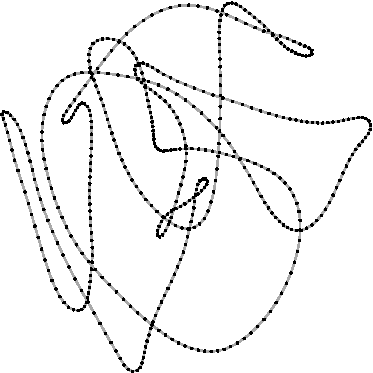
\includegraphics{ResearchTools_files/figure-latex/unnamed-chunk-53-1.pdf}

For the real-world network we can use the following commands. First, the
command \texttt{erdos.renyi.game(500,\ 0.005)} creates a random network,
where each node has a probability of 0.005 to be connected to each other
node.

\begin{Shaded}
\begin{Highlighting}[]
\KeywordTok{plot}\NormalTok{(}\KeywordTok{erdos.renyi.game}\NormalTok{(}\DecValTok{500}\NormalTok{, }\FloatTok{0.005}\NormalTok{), }\DataTypeTok{vertex.label=} \OtherTok{NA}\NormalTok{, }\DataTypeTok{edge.arrow.size=}\FloatTok{0.02}\NormalTok{,}\DataTypeTok{vertex.size =} \FloatTok{0.5}\NormalTok{)}
\end{Highlighting}
\end{Shaded}

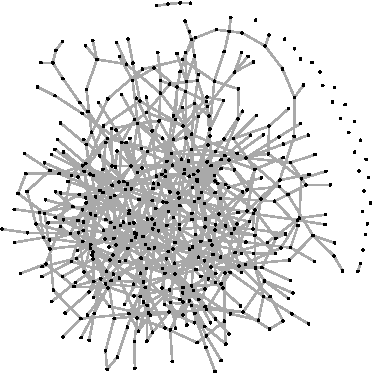
\includegraphics{ResearchTools_files/figure-latex/unnamed-chunk-54-1.pdf}

For the small-world network, we need to rewire the ring network. We can
do by the command \texttt{rewire} as follows:

\begin{Shaded}
\begin{Highlighting}[]
\KeywordTok{plot}\NormalTok{(}\KeywordTok{rewire}\NormalTok{(g_ring,}\KeywordTok{each_edge}\NormalTok{(}\DataTypeTok{prob =} \FloatTok{0.5}\NormalTok{)), }\DataTypeTok{vertex.label=} \OtherTok{NA}\NormalTok{, }\DataTypeTok{edge.arrow.size=}\FloatTok{0.02}\NormalTok{,}\DataTypeTok{vertex.size =} \FloatTok{0.5}\NormalTok{)}
\end{Highlighting}
\end{Shaded}

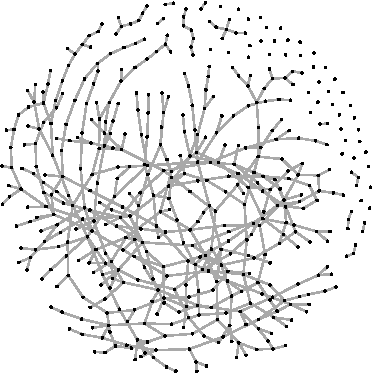
\includegraphics{ResearchTools_files/figure-latex/unnamed-chunk-55-1.pdf}

Note that the probability of rewiring is now 0.5.

Finally, for a power-law we need to invoke an algorithm. In this case
the \texttt{barabasi.game}, where we now create a power-law type of
network with the following underlying formula \(P(k) = k^{-0.5}\).

\begin{Shaded}
\begin{Highlighting}[]
\NormalTok{g_power_law <-}\StringTok{ }\KeywordTok{barabasi.game}\NormalTok{(}\DecValTok{500}\NormalTok{, }\FloatTok{0.5}\NormalTok{)}
\KeywordTok{plot}\NormalTok{(g_power_law, }\DataTypeTok{vertex.label=} \OtherTok{NA}\NormalTok{, }\DataTypeTok{edge.arrow.size=}\FloatTok{0.02}\NormalTok{,}\DataTypeTok{vertex.size =} \FloatTok{0.5}\NormalTok{)}
\end{Highlighting}
\end{Shaded}

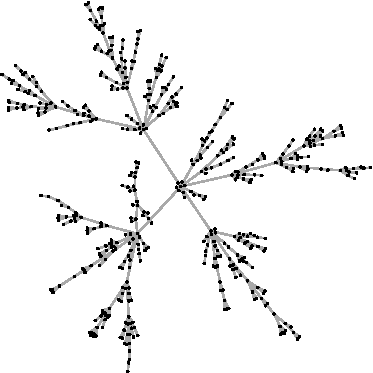
\includegraphics{ResearchTools_files/figure-latex/unnamed-chunk-56-1.pdf}

Note the tree-like structure.

\subsubsection{Reading in networks}\label{reading-in-networks}

Another good but smaller source is the \texttt{igraphdata} package which
actually contains a network of american domestic flights.

Another possibility is to read in the data from a \texttt{.csv} file.
Something like (I took and modified the example from
\url{http://stackoverflow.com/questions/23687806/creating-a-network-graph-using-igraph-in-r}):

\begin{Shaded}
\begin{Highlighting}[]
\CommentTok{# Make up data}
\NormalTok{relations <-}\StringTok{ }\KeywordTok{data.frame}\NormalTok{(}\DataTypeTok{from=}\KeywordTok{c}\NormalTok{(}\StringTok{"Bob"}\NormalTok{, }\StringTok{"Cecil"}\NormalTok{, }\StringTok{"Cecil"}\NormalTok{, }\StringTok{"David"}\NormalTok{, }\StringTok{"David"}\NormalTok{, }\StringTok{"Esmeralda"}\NormalTok{),}
                        \DataTypeTok{to=}\KeywordTok{c}\NormalTok{(}\StringTok{"Alice"}\NormalTok{, }\StringTok{"Bob"}\NormalTok{, }\StringTok{"Alice"}\NormalTok{, }\StringTok{"Alice"}\NormalTok{, }\StringTok{"Bob"}\NormalTok{, }\StringTok{"Alice"}\NormalTok{))}
\CommentTok{# Alternatively, you could read in the data from a similar CSV file as follows:}
\CommentTok{# relations <- read.csv("relations.csv")}

\CommentTok{# Load (DIRECTED) graph from data frame }
\NormalTok{g_relations <-}\StringTok{ }\KeywordTok{graph.data.frame}\NormalTok{(relations, }\DataTypeTok{directed=}\OtherTok{TRUE}\NormalTok{)}
\KeywordTok{plot}\NormalTok{(g_relations)}
\end{Highlighting}
\end{Shaded}

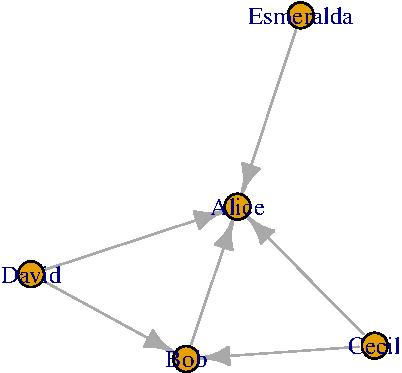
\includegraphics{ResearchTools_files/figure-latex/unnamed-chunk-57-1.pdf}

Note that this only requires a from and to columns in a \texttt{.csv}
file, which resembles trade, commuting, migration and transport networks
(in a gravity-model type of way). The only thing is that we need to
convert this data in a igraph structure with \texttt{graph.data.frame}.

\subsubsection{Sankey networks}\label{sankey-networks}

\begin{Shaded}
\begin{Highlighting}[]
\CommentTok{# Read in the data in a dataframe called Data}
\NormalTok{Data <-}\StringTok{ }\KeywordTok{read.csv}\NormalTok{(}\StringTok{"Migration_Corop_2003.csv"}\NormalTok{, }\DataTypeTok{header=}\OtherTok{TRUE}\NormalTok{,}\DataTypeTok{stringsAsFactors=}\OtherTok{FALSE}\NormalTok{)}
\CommentTok{# We filter some of the data so that our sankey diagram will not be too large}
\NormalTok{Data <-}\StringTok{ }\KeywordTok{filter}\NormalTok{(Data, To <}\StringTok{ }\DecValTok{25}\NormalTok{)}
\NormalTok{Data <-}\StringTok{ }\KeywordTok{filter}\NormalTok{(Data, From <}\StringTok{ }\DecValTok{25}\NormalTok{)}
\CommentTok{# Create a variable for the names of the node (both on the left and right side)}
\NormalTok{DataNames <-}\StringTok{ }\KeywordTok{rep}\NormalTok{(Data$NameFrom[}\DecValTok{1}\NormalTok{:}\DecValTok{8}\NormalTok{], }\DataTypeTok{times=}\DecValTok{2}\NormalTok{)}
\CommentTok{# Create a dataframe of this variable names}
\NormalTok{Names <-}\StringTok{ }\KeywordTok{data.frame}\NormalTok{(DataNames, }\DataTypeTok{stringsAsFactors=}\OtherTok{FALSE}\NormalTok{)}
\CommentTok{# Revalue To and From such that they nicely count up to the number of nodes (Note, we start at index number 0!)}
\NormalTok{Data$To <-}\StringTok{ }\KeywordTok{rep}\NormalTok{(}\DecValTok{8}\NormalTok{:}\DecValTok{15}\NormalTok{, }\DataTypeTok{each=}\DecValTok{8}\NormalTok{)}
\NormalTok{Data$From <-}\StringTok{ }\KeywordTok{rep}\NormalTok{(}\DecValTok{0}\NormalTok{:}\DecValTok{7}\NormalTok{, }\DataTypeTok{times=}\DecValTok{8}\NormalTok{)}

\CommentTok{# Now plot network}
\KeywordTok{sankeyNetwork}\NormalTok{(}\DataTypeTok{Links =} \NormalTok{Data, }\CommentTok{# which dataframe to be used for the flows}
              \DataTypeTok{Nodes =} \NormalTok{Names, }\CommentTok{# which dataframe to be used for the names of the nodes}
              \DataTypeTok{Source =} \StringTok{"From"}\NormalTok{, }\CommentTok{# where do the flows come from (index number)}
              \DataTypeTok{Target =} \StringTok{"To"}\NormalTok{,  }\CommentTok{# where do the flows go to (index number)}
              \DataTypeTok{Value =} \StringTok{"Migrants"}\NormalTok{, }\CommentTok{# the variable that denote the flows from dataframe}
              \DataTypeTok{units =} \StringTok{"Migrants"}\NormalTok{, }\CommentTok{# Which units are the flows (not necessary)}
              \DataTypeTok{NodeID =} \StringTok{"DataNames"}\NormalTok{, }\CommentTok{# Variable that gives the names from the dataframe Names }
              \DataTypeTok{fontSize =} \DecValTok{14}\NormalTok{,  }\CommentTok{# Make things look better}
              \DataTypeTok{nodeWidth =} \DecValTok{40}\NormalTok{) }\CommentTok{# make things look good}
\end{Highlighting}
\end{Shaded}

\hypertarget{htmlwidget-2f5437846f355938e32a}{}

\subsection{Network characteristics}\label{network-characteristics}

So, it is fine that you have a network, but what about the network
characteristics. Well these are easily given once you have a network.

For density, or the completeness of the network, one can look at

\section{\texorpdfstring{\texttt{\{r\}\ \#\ edge\_density(g\_florence\$PADGB)\ \#}}{\{r\} \# edge\_density(g\_florence\$PADGB) \#}}\label{r-edge_densityg_florencepadgb}

\section{}\label{section}

\section{Which give the proportion of the present edges from all
possible edges in the
network.}\label{which-give-the-proportion-of-the-present-edges-from-all-possible-edges-in-the-network.}

\section{}\label{section-1}

\section{The diameter of a network can be retrieved
as:}\label{the-diameter-of-a-network-can-be-retrieved-as}

\section{}\label{section-2}

\section{\texorpdfstring{\texttt{\{r\}\ \#\ diameter(g\_florence\$PADGB)\ \#}}{\{r\} \# diameter(g\_florence\$PADGB) \#}}\label{r-diameterg_florencepadgb}

somewhat more interesting is given by the degree function which gives
the number of connections. For our power-law network this amounts to

\section{\texorpdfstring{\texttt{\{r\}\ \#\ deg\ \textless{}-\ degree(g\_power\_law)\ \#\ deg\ \#}}{\{r\} \# deg \textless{}- degree(g\_power\_law) \# deg \#}}\label{r-deg---degreeg_power_law-deg}

\section{}\label{section-3}

\section{which is not that insightful, but a histogram
is:}\label{which-is-not-that-insightful-but-a-histogram-is}

\section{}\label{section-4}

\section{\texorpdfstring{\texttt{\{r,\ message=FALSE\}\ \#\ hist(deg)\ \#}}{\{r, message=FALSE\} \# hist(deg) \#}}\label{r-messagefalse-histdeg}

Which is typical for a power-law.

The \texttt{degree\_distribution} is insightful here as well

\begin{Shaded}
\begin{Highlighting}[]
\KeywordTok{plot}\NormalTok{(}\KeywordTok{degree_distribution}\NormalTok{(g_power_law, }\DataTypeTok{cumulative =} \OtherTok{TRUE}\NormalTok{))}
\end{Highlighting}
\end{Shaded}

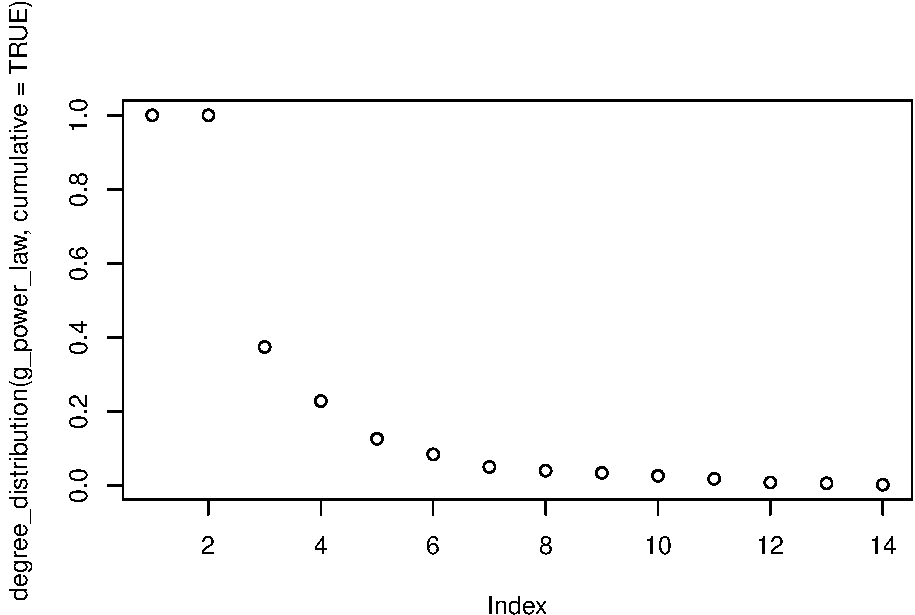
\includegraphics{ResearchTools_files/figure-latex/unnamed-chunk-59-1.pdf}

Finally, we may be interested in the shortest path. This can easily be
retrieved using distances (with underlying Dijkstra's algorithm) as
follows for the Florence network:

\section{\texorpdfstring{\texttt{\{r\}\ \#\ distances(g\_florence\$PADGB)\ \#}}{\{r\} \# distances(g\_florence\$PADGB) \#}}\label{r-distancesg_florencepadgb}

Note that the Pucci family is not in the network and therefore the
distances are set to infinity.

\section{In conclusion}\label{in-conclusion}

To be written


\end{document}
